\documentclass[
  numbers=noenddot,			% Kein . am Ende einer Nummerierung
  bibliography=totoc,       % Literatur im Inhaltsverzeichnis
  listof=totoc,				% Verzeichnisse im Inhaltsverzeichnis
  captions=tableheading,    % Tabellenüberschriften
  fontsize=12pt,
]{scrbook}

\renewcommand{\arrayrulewidth}{1pt}
\usepackage[onehalfspacing]{setspace} % Zeilenabstand 1,5
\usepackage[tableposition=top]{caption} % Tabellen überschrift oben

\usepackage{array}
\usepackage[table]{xcolor}% http://ctan.org/pkg/xcolor
\usepackage[automark]{scrlayer-scrpage}
\setcounter{tocdepth}{4}   %Maximale Gliederungsebene im Inhaltsverziechnis
\setcounter{secnumdepth}{4}   %Maximale Nummerierungsebene im Inhaltsverziechnis
\KOMAoptions{twoside=false}	 	%Einseitige einstellung

% Bei der Klasse "book" ist LaTeX bemüht, den Text auf zwei gegenüberliegenden Seiten auf die gleiche Höhe zu bringen.
% Dies wird dadurch erreicht, dass der Text unter Überschriften oder Zeilenumbrüchen minimal (und nicht sichtbar) variiert wird.
% Bei manchen Dokumenten funktioniert das nicht, da - beispielsweise durch viele Grafiken und wenig Text - nicht genug Spielraum bleibt.
% Das kann dazu führen, dass der Text in einem bestimmten Abstand vom unteren Seitenrand endet und oben noch sehr viel frei ist.
% Durch Aktivieren oder Kommentieren der folgenden Zeilen, kann dieses Verhalten beeinflusst werden.

%%%%%Checken welches besser ist!!!
\flushbottom  	%Der Text aller Seiten ist gleich lang
%\raggedbottom 	%Der Text kann auch unterschiedlich lang sein.

%Abschnittsnummerierungen in Caption und Formelnummerierung
\usepackage{chngcntr}

%Definition der Seitenränder
\usepackage[
  left=4cm,	%Linker Seitenrand (Bindung beachten!!!)
  right=2cm,
  top=3.5cm,
  bottom=3cm
]{geometry}

% Paket float verbessern
\usepackage{scrhack}

%Einstellbarer Zeilenabstand
\usepackage{setspace}

% Warnung, falls nochmal kompiliert werden muss
\usepackage[aux]{rerunfilecheck}

% unverzichtbare Mathe-Befehle
\usepackage[fleqn]{amsmath}
\setlength\mathindent{1cm}%Abstand der Formeln vom linken Seitenrand

% viele Mathe-Symbole
\usepackage{amssymb}

% Erweiterungen für amsmath
\usepackage{mathtools}

% Fonteinstellungen
\usepackage{fontspec}
% Latin Modern Fonts werden automatisch geladen
% Alternativ:
%\setromanfont{Libertinus Serif}
%\setsansfont{Libertinus Sans}
%\setmonofont{Libertinus Mono}
%\recalctypearea % Wenn man andere Schriftarten gesetzt hat,
% sollte man das Seiten-Layout neu berechnen lassen

% deutsche Spracheinstellungen
\usepackage{polyglossia}
\setmainlanguage{german}

\usepackage[
  math-style=ISO,    % ┐
  bold-style=ISO,    % │
  sans-style=italic, % │ ISO-Standard folgen
  nabla=upright,     % │
  partial=upright,   % ┘
  warnings-off={           % ┐
    mathtools-colon,       % │ unnötige Warnungen ausschalten
    mathtools-overbracket, % │
  },                       % ┘
]{unicode-math}

% traditionelle Fonts für Mathematik
\setmathfont{Latin Modern Math}
% Alternativ:
%\setmathfont{Libertinus Math}

\usepackage{amsmath}
\usepackage{amssymb}\setmathfont{XITS Math}[range={scr, bfscr}]

\setmathfont{XITS Math}[range={scr, bfscr}]
\setmathfont{XITS Math}[range={cal, bfcal}, StylisticSet=1]
\setlength{\delimitershortfall}{-1sp}

%\setmathfont{Cambria Math}

% Zahlen und Einheiten
\usepackage[
  locale=DE,                   % deutsche Einstellungen
  separate-uncertainty=true,   % immer Fehler mit \pm
  per-mode=symbol-or-fraction, % / in inline math, fraction in display math
  range-phrase = ~\text{bis}~ ,
]{siunitx}

% richtige Anführungszeichen
\usepackage[autostyle]{csquotes}

% schöne Brüche im Text
\usepackage{xfrac}

% Standardplatzierung für Floats einstellen
% Die Reihenfolge der Befehle bestimmt was Priorität hat
% tb!hp bedeutet versuche eine Grafik oder Tabelle zuerst oben auf der Seite zu plazieren
% wenn das nicht geht versuche sie unten auf der Seite zu platzieren
% wenn das auch nicht geht setze sie genau an die Stelle wo sie im Text vorkommt
% und im Worst-Case schiebe sie auf eine separate Seite
\usepackage{float}
\floatplacement{figure}{tb!hp}
\floatplacement{table}{tb!hp}

% Floats innerhalb einer Section halten
\usepackage[
  section, % Floats innerhalb der Section halten
  below,   % unterhalb der Section aber auf der selben Seite ist ok
]{placeins}

% Seite drehen für breite Tabellen: landscape Umgebung
\usepackage{pdflscape}

% Captions schöner machen.
\usepackage[
  labelfont=bf,        % Tabelle x: Abbildung y: ist jetzt fett
  font=small,          % Schrift etwas kleiner als Dokument
  width=0.9\textwidth, % maximale Breite einer Caption schmaler
  labelsep=colon,      % Doppelpunkt als Trenner
  format=plain,%Beschriftung wird als Absatz gesetzt
  indention=0pt,%Einzug der Beschriftung ist 0
]{caption}



% subfigure, subtable, subref
\usepackage{subcaption}

% Grafiken können eingebunden werden
\usepackage{graphicx}

%Erstellen von Plots
\usepackage{pgfplots}
\pgfplotsset{compat=1.14}
\usetikzlibrary{calc}

% Schaltpläne
\usepackage[european,siunitx,straightvoltages]{circuitikz}

% schöne Tabellen
\usepackage{booktabs}

% Verbesserungen am Schriftbild
\usepackage{microtype}

% Literaturverzeichnis
\usepackage[
  backend=biber,
  isbn=false,
  style=numeric
]{biblatex}

% Quellendatenbank
\addbibresource{bibliography.bib}

%Mehr Einstellungsmöglichkeiten bei Aufzählungen
\usepackage{enumitem}

%Für Einbinden von z.B. pdf_tex mit relativem Pfad
\usepackage{import}

%Konfiguration der Todos
\usepackage[prependcaption]{todonotes}			%Für Todos eingeblendet
%\usepackage[prependcaption,disable]{todonotes}	%Für Todos ausgeblendet

%Für Programmlistings
\usepackage{listings}

%Für MATLAB Listings
\usepackage[numbered,framed]{matlab-prettifier}

%Setzen von Optionen zur Darstellung von Listings
%Quelle: https://en.wikibooks.org/wiki/LaTeX/Source_Code_Listings (angepasst)
\lstdefinestyle{C}{
	backgroundcolor=\color{white},     % choose the background color; you must add \usepackage{color} or \usepackage{xcolor}; should come as last argument
	basicstyle=\footnotesize\ttfamily, % the size of the fonts that are used for the code
	breakatwhitespace=false,           % sets if automatic breaks should only happen at whitespace
	breaklines=true,                   % sets automatic line breaking
	captionpos=b,                      % sets the caption-position to bottom
	commentstyle=\itshape\color{purple!40!black},    % comment style
	deletekeywords={...},              % if you want to delete keywords from the given language
	escapeinside={\%*}{*)},            % if you want to add LaTeX within your code
	extendedchars=true,                % lets you use non-ASCII characters; for 8-bits encodings only, does not work with UTF-8
	frame=single,	                   % adds a frame around the code
	keepspaces=true,                   % keeps spaces in text, useful for keeping indentation of code (possibly needs columns=flexible)
	keywordstyle=\bfseries\color{green!40!black},       % keyword style
	language=C,                 	   % the language of the code
	morekeywords={*,...},              % if you want to add more keywords to the set
	numbers=left,                      % where to put the line-numbers; possible values are (none, left, right)
	numbersep=5pt,                     % how far the line-numbers are from the code
	numberstyle=\tiny\color{gray},     % the style that is used for the line-numbers
	rulecolor=\color{black},           % if not set, the frame-color may be changed on line-breaks within not-black text (e.g. comments (green here))
	showspaces=false,                  % show spaces everywhere adding particular underscores; it overrides 'showstringspaces'
	showstringspaces=false,            % underline spaces within strings only
	showtabs=false,                    % show tabs within strings adding particular underscores
	stepnumber=1,                      % the step between two line-numbers. If it's 1, each line will be numbered
	stringstyle=\color{orange},        % string literal style
	identifierstyle=\color{blue},
	tabsize=2,	                   	  % sets default tabsize to 2 spaces
	title=\lstname                    % show the filename of files included with \lstinputlisting; also try caption instead of title
}


\lstdefinestyle{C++}{
	backgroundcolor=\color{white},   % choose the background color; you must add \usepackage{color} or \usepackage{xcolor}; should come as last argument
	basicstyle=\footnotesize\ttfamily,        % the size of the fonts that are used for the code
	breakatwhitespace=false,         % sets if automatic breaks should only happen at whitespace
	breaklines=true,                 % sets automatic line breaking
	captionpos=b,                    % sets the caption-position to bottom
	commentstyle=\itshape\color{purple!40!black},    % comment style
	deletekeywords={...},            % if you want to delete keywords from the given language
	escapeinside={\%*}{*)},          % if you want to add LaTeX within your code
	extendedchars=true,              % lets you use non-ASCII characters; for 8-bits encodings only, does not work with UTF-8
	frame=single,	                   % adds a frame around the code
	keepspaces=true,                 % keeps spaces in text, useful for keeping indentation of code (possibly needs columns=flexible)
	keywordstyle=\bfseries\color{green!40!black},       % keyword style
	language=C++,                 	   % the language of the code
	morekeywords={*,...},            % if you want to add more keywords to the set
	numbers=left,                    % where to put the line-numbers; possible values are (none, left, right)
	numbersep=5pt,                   % how far the line-numbers are from the code
	numberstyle=\tiny\color{gray},   % the style that is used for the line-numbers
	rulecolor=\color{black},         % if not set, the frame-color may be changed on line-breaks within not-black text (e.g. comments (green here))
	showspaces=false,                % show spaces everywhere adding particular underscores; it overrides 'showstringspaces'
	showstringspaces=false,          % underline spaces within strings only
	showtabs=false,                  % show tabs within strings adding particular underscores
	stepnumber=1,                    % the step between two line-numbers. If it's 1, each line will be numbered
	stringstyle=\color{orange},      % string literal style
	identifierstyle=\color{blue},
	tabsize=2,	                     % sets default tabsize to 2 spaces
	title=\lstname                   % show the filename of files included with \lstinputlisting; also try caption instead of title
}


\lstdefinestyle{Java}{
	backgroundcolor=\color{white},   % choose the background color; you must add \usepackage{color} or \usepackage{xcolor}; should come as last argument
	basicstyle=\footnotesize\ttfamily,        % the size of the fonts that are used for the code
	breakatwhitespace=false,         % sets if automatic breaks should only happen at whitespace
	breaklines=true,                 % sets automatic line breaking
	captionpos=b,                    % sets the caption-position to bottom
	commentstyle=\itshape\color{purple!40!black},    % comment style
	deletekeywords={...},            % if you want to delete keywords from the given language
	escapeinside={\%*}{*)},          % if you want to add LaTeX within your code
	extendedchars=true,              % lets you use non-ASCII characters; for 8-bits encodings only, does not work with UTF-8
	frame=single,	                   % adds a frame around the code
	keepspaces=true,                 % keeps spaces in text, useful for keeping indentation of code (possibly needs columns=flexible)
	keywordstyle=\bfseries\color{green!40!black},       % keyword style
	language=Java,                 	   % the language of the code
	morekeywords={*,...},            % if you want to add more keywords to the set
	numbers=left,                    % where to put the line-numbers; possible values are (none, left, right)
	numbersep=5pt,                   % how far the line-numbers are from the code
	numberstyle=\tiny\color{gray},   % the style that is used for the line-numbers
	rulecolor=\color{black},         % if not set, the frame-color may be changed on line-breaks within not-black text (e.g. comments (green here))
	showspaces=false,                % show spaces everywhere adding particular underscores; it overrides 'showstringspaces'
	showstringspaces=false,          % underline spaces within strings only
	showtabs=false,                  % show tabs within strings adding particular underscores
	stepnumber=1,                    % the step between two line-numbers. If it's 1, each line will be numbered
	stringstyle=\color{orange},      % string literal style
	identifierstyle=\color{blue},
	tabsize=2,	                     % sets default tabsize to 2 spaces
	title=\lstname                   % show the filename of files included with \lstinputlisting; also try caption instead of title
}


\lstdefinestyle{ML}{
	basicstyle         = \mlttfamily,
	language           = Matlab,
	style              = Matlab-editor,
	escapechar         = `,
	mlshowsectionrules = true,
	captionpos=b,
}

% Hyperlinks im Dokument
\usepackage[
 hidelinks,       %Keine Markierung um den Link
 unicode,        % Unicode in PDF-Attributen erlauben
 pdfusetitle,    % Titel, Autoren und Datum als PDF-Attribute
 pdfcreator={},  % ┐ PDF-Attribute säubern
 pdfproducer={}, % ┘
]{hyperref}

%Abkürzungsverzeichnis
\usepackage[nopostdot,style=super,nonumberlist,toc]{glossaries}
%Anpassen der Breite der zweiten Spalte um einen zu frühen Zeilenumbruch zu verhindern
\setlength{\glsdescwidth}{0.8\textwidth}
\newglossary[slg]{symbols}{sym}{sbl}{Symbolverzeichnis}%Definition Symbolverzeichnis
\loadglsentries{glossary.tex}%Einbinden de Glossars
\makeglossaries

% erweiterte Bookmarks im PDF
\usepackage{bookmark}

% Trennung von Wörtern mit Strichen
\usepackage[shortcuts]{extdash}

%Kopf/Fußzeile=====================
\KOMAoptions{headsepline=true}
\KOMAoptions{footsepline=true}
%\rohead*{\textnormal{\headmark}}
%\lehead*{\textnormal{\headmark}}
\cofoot*{\pagemark}
\cefoot*{\pagemark}
\rofoot*{}
\lefoot*{}

\newpairofpagestyles{kapitel}{%Kapitelseiten formatieren
	\clearpairofpagestyles
	\KOMAoptions{headsepline=false}
	\KOMAoptions{footsepline=true}
	%\lofoot*{\footnotesize\textnormal{}}
	\cofoot*{\pagemark}
	\cefoot*{\pagemark}
}
\renewcommand*{\chapterpagestyle}{kapitel}

%Kopf/Fußzeile=====================

%%Anpassen der Abbildungs- und Tabellennummerierung========

\counterwithin*{figure}{chapter}

\renewcommand{\thefigure}{%
	\ifnum\value{chapter}=0
	\arabic{figure}%
	\else
	\thechapter-\arabic{figure}%
	\fi
}



\counterwithin*{table}{chapter}


\renewcommand{\thetable}{%
 \ifnum\value{chapter}=0
  \arabic{table}%
 \else
   \thechapter-\arabic{table}%
\fi
}

\counterwithin*{equation}{chapter}



\renewcommand{\theequation}{%
 \ifnum\value{chapter}=0
  \arabic{equation}%
 \else
   \thechapter-\arabic{equation}%
 \fi
}

%%Da die Bezeichnung nun länger ist, muss der Abstand in den Verzeichnissen angepasst werden
%\makeatletter
%\renewcommand*\l@figure{\@dottedtocline{1}{1.5em}{4.2em}}% 3.2em statt 2.3em
%\let\l@table\l@figure %\makeatother
%%Ende Anpassen der Abbildungs- und Tabellennummerierung========

%Komplexe Zahlen
\newcommand{\komp}[2]{\underline{#1}_\text{#2}}

%zeichen
\newcommand{\flet}[2]{#1_\text{#2}}

%Gleiche Linienstärke in circutikz für Leitungen und Bipoles
\ctikzset{bipoles/thickness=1}

%Einheit für Jahr
\DeclareSIUnit[number-unit-product = \,]{\year}{yr}

% Werden Funktionen in LaTeX direkt geplottet, kann dies zu einer sehr langen Kompilezeit führen.
% Aus diesem Grund wird die Anzahl der zu berechnenden Datenpunkte in einer Variable definiert und kann
% so bei Bedarf reduziert, und für die Endfassung entsprechend erhöht werden.
\newcommand{\NumOfSampels}{1000}%Anzahl der Samples für Plots



\begin{document}
\newgeometry{left=3.5cm, right=2.5cm, top=2cm, bottom=2cm}%Seitenränder der Titelseite anpassen
\begin{titlepage}
	\setlength{\parindent}{0pt}%Einrückung auf Titelseite verhindern
	\begin{figure}
		
\includegraphics[height=1.4cm]{content/Grafiken/H-BRS_Logo}
		\hfill
		
	\end{figure}
	\vspace{1cm}
	\begin{onehalfspace}
		 Fachbereich Ingenieurwissenschaften\\
		 und Kommunikation (IWK)\\
		Studiengang Elektrotechnik M. Eng.\\
		Vertiefungsrichtung Elektronische Systementwicklung 
		\vspace{2cm}
		\begin{center}
			\begin{singlespacing}
				{\large\textsf{Master-Thesis}\par}
				\vspace{1mm}
				{\huge\textbf{\textsf{
					Netzdienliche Wasserstoff-Elektrolysegleichrichter: Eine Analyse von IAF und 1/3 PWM PFC Rectifier in der Leistungsklasse 400 kVA
				}}\par}
			\end{singlespacing}
		\end{center}
		\vfill
		Vorgelegt von:\\
		Jonas Heinemann\\
		Cecilienstraße 28\\
		53840 Troisdorf\\
		Tel. 015783841858\\
		\href{mailto:heinemann.jonas@gmx.de}{heinemann.jonas@gmx.de}\\
		Matr.-Nr. 9031399
		\begin{table}
			\begin{tabular}{@{}ll}
				Erstprüfer:  & Prof. Dr.-Ing. Marco Jung\\
				Zweitprüfer: & Prof. Dr. Heinrich Richard Salbert\\
			\end{tabular}
		\end{table}
	\end{onehalfspace}
	Troisdorf, den 08.03.2024
\end{titlepage}

\restoregeometry%Seitenränder auf defaultwert

\thispagestyle{empty}
\section*{Erklärung zur Master-Thesis}
„Ich versichere hiermit, die von mir vorgelegte Arbeit selbstständig verfasst zu haben. Alle Stellen, die wörtlich oder sinngemäß aus veröffentlichten oder nicht veröffentlichten Arbeiten anderer entnommen sind, habe ich als entnommen kenntlich gemacht. Sämtliche Quellen und Hilfsmittel, die ich für die Arbeit benutzt habe, sind angegeben. Die Arbeit hat mit gleichem Inhalt bzw. in wesentlichen Teilen noch keiner anderen Prüfungsbehörde vorgelegen.

Mir ist bewusst, dass sich die Hochschule vorbehält, meine Arbeit auf plagiierte Inhalte hin zu überprüfen und dass das Auffinden von plagiierten Inhalten zur Nichtigkeit der Arbeit, zur Aberkennung des Abschlusses und zur Exmatrikulation führen können.“
\vspace{3cm}


\noindent\parbox[t]{5cm}{\underline{\hspace{5cm}}\\\noindent Ort, Datum}%
\hfill%
\noindent\parbox[t]{5cm}{\noindent\underline{\hspace{5cm}}\\\noindent Unterschrift}%

\frontmatter%Beginn des Vorspanns
\pagenumbering{Roman}%Große römische Seitennummerierung
\chapter{Kurzfassung}
Um in Zukunft unabhängiger von Importen zu sein und die Energieversorgung nachhaltiger zu gestalten, hat die Bundesregierung das Ziel für die Erzeugung von grünem Wasserstoff durch Elektrolyse von fünf auf zehn Gigawatt Leistung im Jahr 2030 angehoben. Davon sollen drei Gigawatt systemdienlich sein \cite{BMWKH2}. Dies zeigt, wie wichtig es ist, die Elektrolyse für zukünftige Szenarien vorzubereiten.
Um darüber hinaus das Ziel rein erneuerbarer Energien im Stromnetz zu erreichen, ist es notwendig, die Anforderungen an größere Lasten zu verändern. Dies betrifft die Systemdienstleistungen, die bisher vor allem von zentralen Großkraftwerken erbracht werden. Zukünftig sollen in Deutschland Wasserstoff-Elektrolyseanlagen in der Leistungsklasse von mehreren Megawatt aufgebaut werden, die viele Möglichkeiten bieten, das Stromnetz durch Dynamik und Regelung zu unterstützen. Daher werden in dieser Arbeit Stromrichter für die Anwendung der Wasserstoffelektrolyse untersucht, die innovative Ansätze und eine optimierte Betriebsführung ermöglichen. Anhand einer Vorauswahl werden die relevanten Topologien auf den \gls{IAF} und \gls{B6PFC} eingegrenzt, diese werden anschließend detailliert untersucht und durch Simulationsmodelle charakterisiert.\\
Zum abschließenden Vergleich der Modelle erfolgt eine Bewertung anhand des Bedarfs an induktiven und Halbleiterbauelementen sowie der Halbleiterverluste aus dem Simulationsmodell. Diese Größen werden in den einzelnen Kategorien normiert und über Gewichtungsfaktoren zu einer Gesamtbewertung zusammengefasst. Darüber hinaus wird ein Ausblick auf zukünftige Schritte wie die Optimierung der Halbleitermodelle durch Messungen und den Aufbau eines Demonstrators gegeben.

\tableofcontents%Inhaltsverzeichnis
\listoffigures%Abbildungsverzeichnis
\listoftables%Tabellenverzeichnis

\printglossary[type=\acronymtype,title=Abkürzungsverzeichnis] %Abkürzungsverzeichnis


\clearpage
\mainmatter 				%Beginn des Haupteils (arabische Seitennummerierung)
\chapter{Einleitung}
Um die Klimaschutzziele zu erreichen, wird eine Vielzahl von Maßnahmen notwendig sein, die nur im Zusammenspiel zum Erfolg führen können. Ein großes Problem bei der Nutzung erneuerbarer Energien ist deren Volatilität, daher sind deutlich größere Speichermöglichkeiten erforderlich. Ein Medium für die langfristige Speicherung und den Transport von Energie bietet Wasserstoff, der auf unterschiedliche Weise gewonnen werden kann und vielfältige Einsatzmöglichkeiten bietet. In der Industrie wird Wasserstoff bereits heute in großem Umfang eingesetzt. In den meisten Fällen wird er jedoch durch Dampfreformierung direkt am Einsatzort aus Erdgas gewonnen. Zukünftig kann er durch den Einsatz von Elektrolysezellen mit erneuerbaren Energien nachhaltig erzeugt werden \cite{Elektrolyse}. 
\section{Stand der Technik}
 Die Entwicklung der Elektrolyse schreitet sehr schnell voran und in den nächsten Jahren sind Veränderungen zu erwarten, die auch die Stromversorgung betreffen. Insbesondere der Trend zu höheren Spannungsklassen ermöglicht eine Kostenreduktion auf Seiten der Leistungselektronik. Die optimale Auslegung der Elektrolyseanlage hängt jedoch von vielen anwendungsspezifischen Parametern wie z.~B. der Betriebsführung ab. Insbesondere die Entwicklung des Strompreises und die Netzstabilität in der Zukunft können die Amortisation stark beeinflussen. Durch Gleichrichter, die das Netz unterstützen, anstatt es z.~B. durch Blindleistungsbezug zu belasten, können Elektrolyseure ohne zusätzliche Kompensationsanlagen günstiger betrieben werden. Darüber hinaus kann durch Frequenzstabilisierung und andere \gls{SDL} zusätzliche Vergütung generiert werden. \\
Die \gls{IRENA} hat in ihrem Bericht über die Kostenentwicklung der Elektrolyse im Jahr 2020 den Anteil der Kosten für die Stromversorgung für \gls{PEM}-Elektrolyseure mit 29 bis 38 Prozent angegeben. Wobei die Elektrolysezellen selbst weniger als die Hälfte der Kosten ausmachen. Darüber hinaus werden als mögliche Faktoren zur Senkung der Gleichrichterkosten Skaleneffekte, die Standardisierung von Komponenten sowie die Beteiligung von Unternehmen aus der Elektronikindustrie anstelle von Elektrolyseurherstellern genannt \cite{IRENA2020}.\\ 
	\begin{figure} 
		\centering
		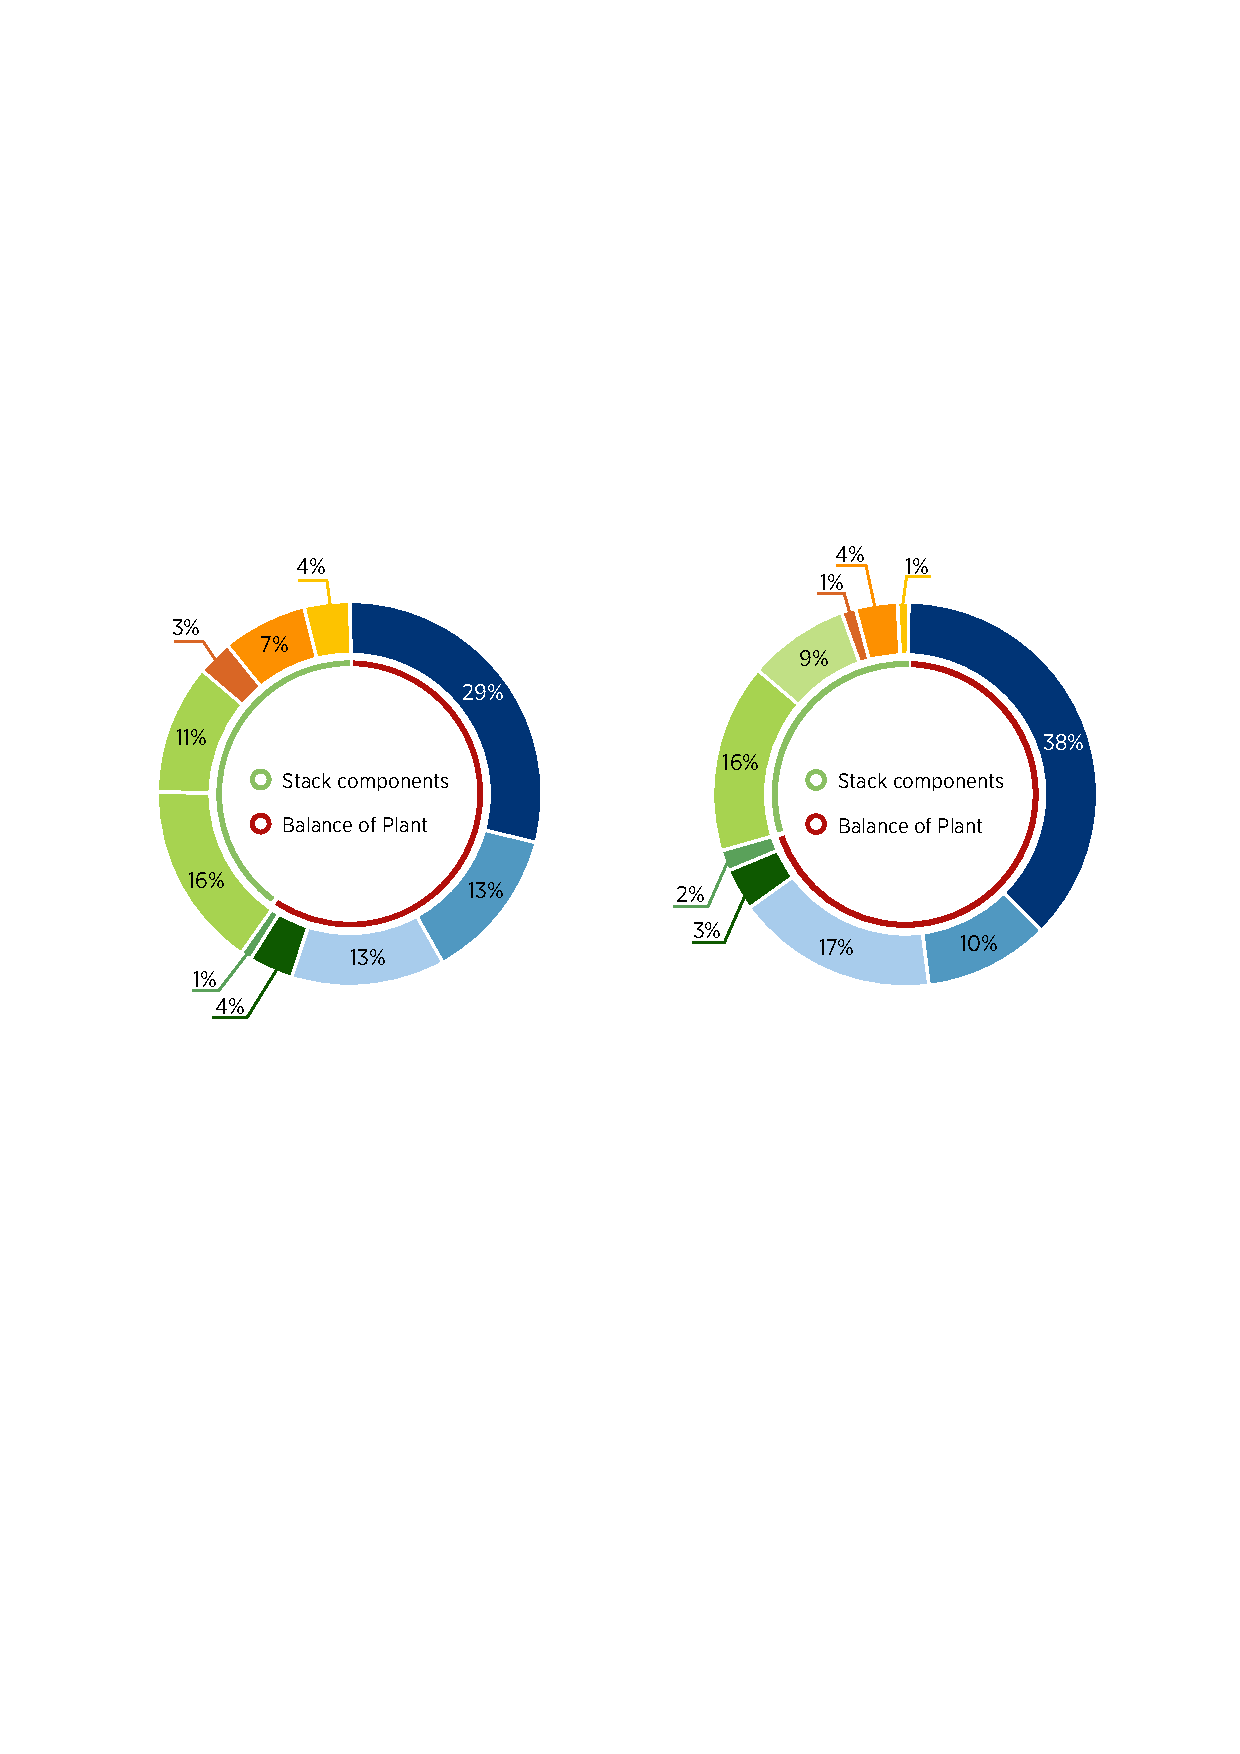
\includegraphics[width=1\linewidth]{content/Grafiken/ElyCost}
		\caption[Systemkosten PEM Elektrolyse]{Systemkosten \gls{PEM} Elektrolyse links 10 MW pro Jahr, rechts 1 GW pro Jahr \cite{IRENA2020}}
		\label{fig:elycost}
	\end{figure}
Die Abb. \ref{fig:elycapacity} zeigt zudem, dass der Ausbau der Elektrolyse in den letzten Jahren enorm zugenommen hat und in Zukunft noch deutlich zunehmen wird. Die weltweite Leistung hat gerade den Gigawatt-Bereich erreicht und soll allein in Deutschland bis 2030 auf mindestens zehn Gigawatt ausgebaut werden.\\
	\begin{figure}
		\centering
		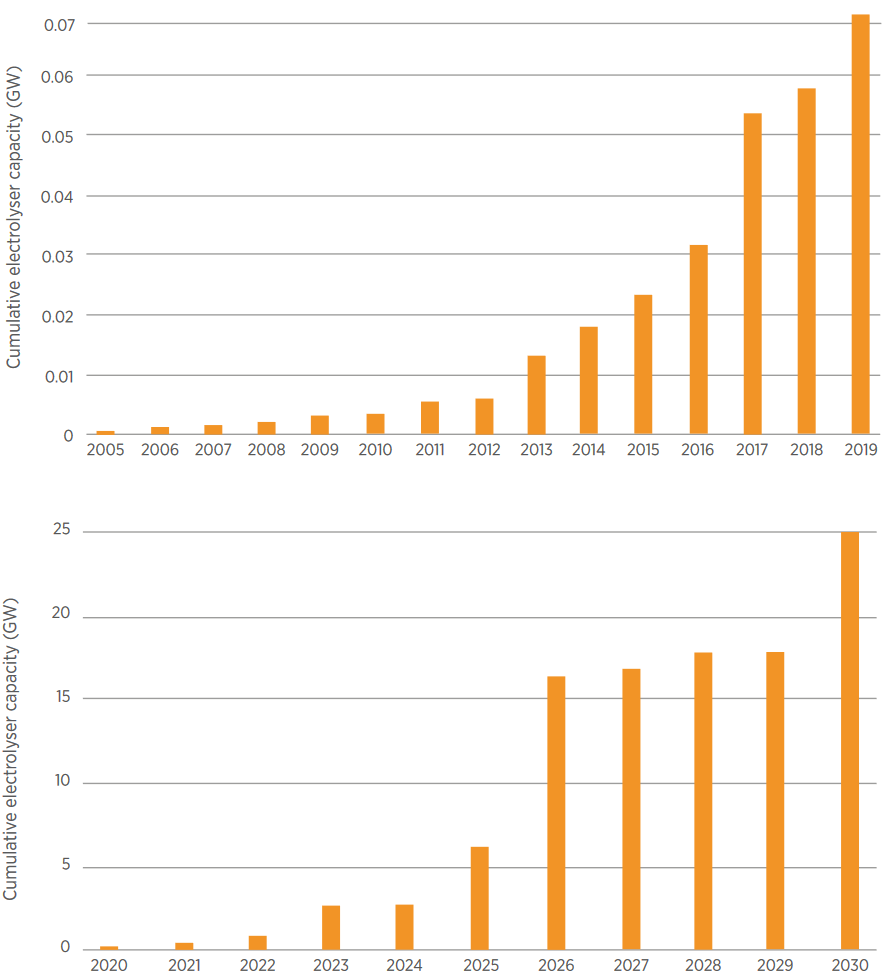
\includegraphics[width=0.7\linewidth]{content/Grafiken/Ely_Capacity}
		\caption[Elektrolyse Kapazität bis 2030]{Elektrolysekapazität Stand 2020 mit Ausblick bis 2030 \cite{IRENA2020}}
		\label{fig:elycapacity}
	\end{figure}
Ein grundlegendes Unterscheidungsmerkmal für Gleichrichterschaltungen ist die Umsetzung als Dioden/Thyristor oder aktiver Gleichrichter. In Abbildung \ref{fig:thyristor} ist ein Beispiel für einen 6-pulsigen Thyristor-Gleichrichter zu sehen . 
	\begin{figure} 
		\centering
		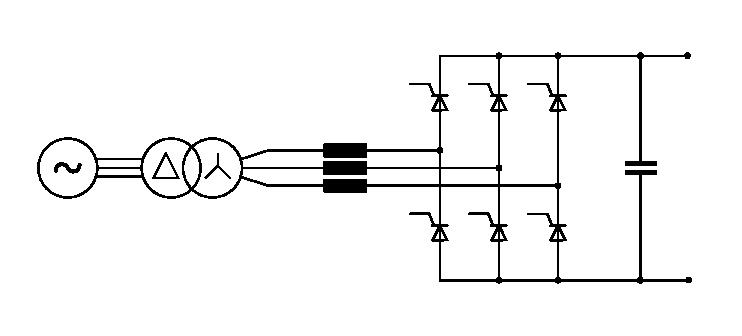
\includegraphics[width=0.9\linewidth]{content/Grafiken/Thyristor}
		\caption{Aufbau eines Thyristor-Gleichrichters}
		\label{fig:thyristor}
	\end{figure}
Thyristorgleichrichter haben aufgrund ihrer kompakten Bauform eine höhere Leistungsdichte und können in großen Stückzahlen kostengünstig produziert werden. Zudem gibt es bereits zahlreiche Lösungen für unterschiedliche Anwendungen. Eine Übersicht mit Bewertung geeigneter Gleichrichter für den Einsatz in Elektrolyseanlagen wurde von Mengxing Chen et al. erstellt \cite{HydrogenElectronicTopologies}. Aufgrund der Blindleistung von Thyristorschaltungen benötigen sie zusätzliche STATCOM-Anlagen zur Kompensation am Netzanschlusspunkt. Um eine bessere Performance zu ermöglichen, können zusätzlich Zerhacker (Chopper) erforderlich sein. Durch die 12-pulsige Anordnung und die höhere Ausgangsspannung ist der Aufbau des Netztransformators außerdem komplexer \cite{HydrogenRectInf}. Aktive Gleichrichter zeichnen sich durch ihre Netzqualität, Sie können einen konstanten Leistungsfaktor erreichen und benötigen daher keine Kompensationsanlagen. Außerdem kann die Verzerrung \gls{THD} unter 5 \% liegen, so dass der Filteraufwand geringer ist. Durch Multi-Level-Topologien können Halbleiter besser ausgenutzt und der Wirkungsgrad erhöht werden. Innovative Konzepte erfordern jedoch einen höheren Entwicklungsaufwand und die Zuverlässigkeit ist schwieriger zu gewährleisten. Einen Überblick über die Eigenschaften gibt die Tabelle \ref{tab:thyVSafe}.\\
	\begin{table}
		\centering
		\caption{Vergleich Thyristor-Gleichrichter und aktiver Gleichrichter}
		\label{tab:thyVSafe}
		\begin{tabular}{|c|c|} 
			\hline
			\textbf{Diode / Thyristor} & \textbf{Aktiver Gleichrichter} \\
			\hline
			Hohe Leistungsdichte & Einheitlicher Leistungsfaktor \\
			\hline
			Geringe Halbleiterkosten & <5 \% \gls{THD} \\
			\hline
			Vorgefertigte Lösungen & Mehr Level Topologien  \\
			\hline
			Benötigt STATCOM &  \gls{SDL} möglich \\
			\hline
			Zusätzlicher Zerhacker (Chopper) ggf  nötig & Innovative Lösungen \\
			\hline
			Komplexer Transformator & Aufwändigere Entwicklung \\
			\hline
		\end{tabular}
	\end{table}
Für Gleichrichter im Megawattbereich sind Thyristorschaltungen die am häufigsten verwendete Lösung, da diese Halbleiter aufgrund ihrer langjährigen Entwicklung sehr zuverlässig und robust sind. Zur Optimierung von Blindleistung und \gls{THD} werden meist 12-Puls-Schaltungen verwendet, dies wird durch Verschieben und Überlagern der einzelnen Schaltungen erreicht. Bei Reduzierung der Ausgangsleistung muss jedoch der Zündwinkel so weit vergrößert werden, dass eine externe Blindleistungskompensation erforderlich wird \cite{HydrogenElectronicTopologies}. Daher sind diese Schaltungen nur für Anlagen geeignet, die die meiste Zeit mit hoher Leistung betrieben werden. Ein weiterer Nachteil ist, dass die Elektrolyseure mit gleicher Leistung und Ausgangsspannung betrieben werden müssen. Dadurch ist zum einen eine Wartung an einzelnen Stacks sowie der Austausch einzelner Stacks nicht möglich. Dies stellt bei großen Anlagen ein Problem dar, da die Spannung der Stacks über die Laufzeit ansteigt und ein neuer Stack eine andere Spannung benötigt.\\
Aktuelle Forschungsergebnisse zu Hochleistungsgleichrichtern für die Elektrolyse sind in \cite{HydrogenRectifier} dargestellt. Hier zeigt sich, dass insbesondere bei höheren Ausgangsspannungen neue Konzepte mit integrierter Blindleistungskompensation wie der Vienna-Gleichrichter gut geeignet sind \cite{HydrogenRectifier}.
%\pagebreak
\section{Ziel der Arbeit}
Ziel ist es, die beiden ausgewählten Stromrichtertopologien (\gls{IAF} und \gls{B6PFC}) anhand detaillierter Simulationen unter vorgegebenen Randbedingungen zu vergleichen, um eine eindeutige Bewertung vornehmen zu können. Dazu werden zunächst die Randbedingungen der Schnittstellen Elektrolyseur und Stromnetz definiert, um diese in einer Simulation mit Matlab und der Erweiterung PLECS abzubilden. Durch die Modellierung der Halbleiter kann die Verlustleistung und damit der Wirkungsgrad und indirekt der Kühlaufwand abgeschätzt werden. Zusätzlich kann durch die in den magnetischen Komponenten gespeicherte Energie deren Größe und Kosten abgeschätzt werden, da diese den größten Anteil an den Gesamtkosten eines Umrichters ausmachen. Weitere Komponenten wie Treiberschaltungen und benötigte Kapazitäten spielen bei der Bewertung eine untergeordnete Rolle. Um die Bereitstellung von Systemdienstleistungen zu berücksichtigen, wird die Verlustleistung ohne und mit einer Phasenverschiebung von 30 Grad betrachtet. Anschließend erfolgt eine Gesamtbewertung durch Gewichtungsfaktoren der einzelnen Kategorien.
\chapter{Grundlagen}
Die Leistungselektronik ist ein komplexes Thema das im Grunde mit dem Beginn der Elektrizität beginnt, die Wandlung und Übertragung von Strom stellte die ersten großen Hindernisse dar. Insbesondere die Entscheidung zwischen Wechsel- und Gleichspannung in den Übertragungs- und Verteilnetzen stellte eine erste Große Debatte dar. Durch die Weiterentwicklung in der Halbleitertechnik zeigt sich, dass Gleichstromtechnik insbesondere bei langen Übertragungsstrecken Vorteile gegenüber der verbreiteteren Wechselstromtechnik besitzt. Um die Anforderungen und Zusammenhänge verstehen zu können, werden Details zur Elektrolyse, zu Stromrichtern sowie Komponenten und der verwendeten Simulationsumgebung dargestellt.

\section{Wasserstoff-Elektrolyse}
\label{sec:Elektrolyse}
Unter Wasserstoff-Elektrolyse versteht man grundlegend die Funktion Wasser in seine Bestandteile Wasserstoff und Sauerstoff zu spalten. Die verbreitetste Variante ist die \gls{AEL}, welche bereits im großen Maßstab von bis zu zwei Giga Watt eingesetzt wird \cite{2GWely}. Des weiteren wird viel Potential in der Weiterentwicklung der \gls{PEM} Elektrolyse gesehen, da diese durch einen simpleren Aufbau und höhere Stromdichten bessere Skalierbarkeit bieten kann. Außerdem wird die \gls{HTEL} verwendet, wenn sich die Nutzung von Prozess technischer Abwärme anbietet, wodurch der Gesamtwirkungsgrad steigt \cite{Elektrolyse}.\\
Das Prinzip der \gls{AEL} wird, im Gegensatz zur neueren \gls{PEM}, Elektrolyse bereits seit langer Zeit verwendet und optimiert. Die \gls{AEL} benötigt in der Regel eine wässrige KOH-Lauge und kann durch Reihenschaltung der Zellen Wasserstoff und Sauerstoff mit erhöhtem Druck von Beispielsweise 30 Bar bereitstellen. Die Entwicklung und insbesondere Steigerung der Stromdichte und Effizienz brachte in den letzten Jahren jedoch keine großen Änderungen. Der Spannungswirkungsgrad liegt zwischen 62 und 82 Prozent \cite{NOWH2}.\\
Die \gls{PEM} Elektrolyse bietet Vorteile durch erhöhte Stromdichte, bei größeren Anlagen spart dies unter anderem Platzbedarf, außerdem ist zu erwarten, dass Druckelektrolyse bis 100 Bar möglich ist. Jedoch gibt es noch Optimierungsbedarf bei der  Langlebigkeit der Membranen und der benötigten Edelmetalle \cite{NOWH2}. \\
Die \gls{HTEL} nutzt die Vorteile durch höhere Temperatur, welche auf der Seite der Thermodynamik Vorteile für die Elektrische-Effizienz bringen, jedoch hohe Anforderungen an die verwendeten Materialien stellen. Daher ist die Festoxid Elektrolyse noch in einer Grundlagenforschung im Laborstadium. Da fast alle Festoxid-Zellen umkehrbare Eigenschaften besitzen ist das Interesse an ihnen besonders groß, dies ermöglicht die direkte Rückverstromung des Wasserstoffs. Jedoch wird hier ebenfalls noch eine Materialoptimierung sowie Verbesserung der Langzeiteigenschaften benötigt.\\

\begin{figure}
	\centering
	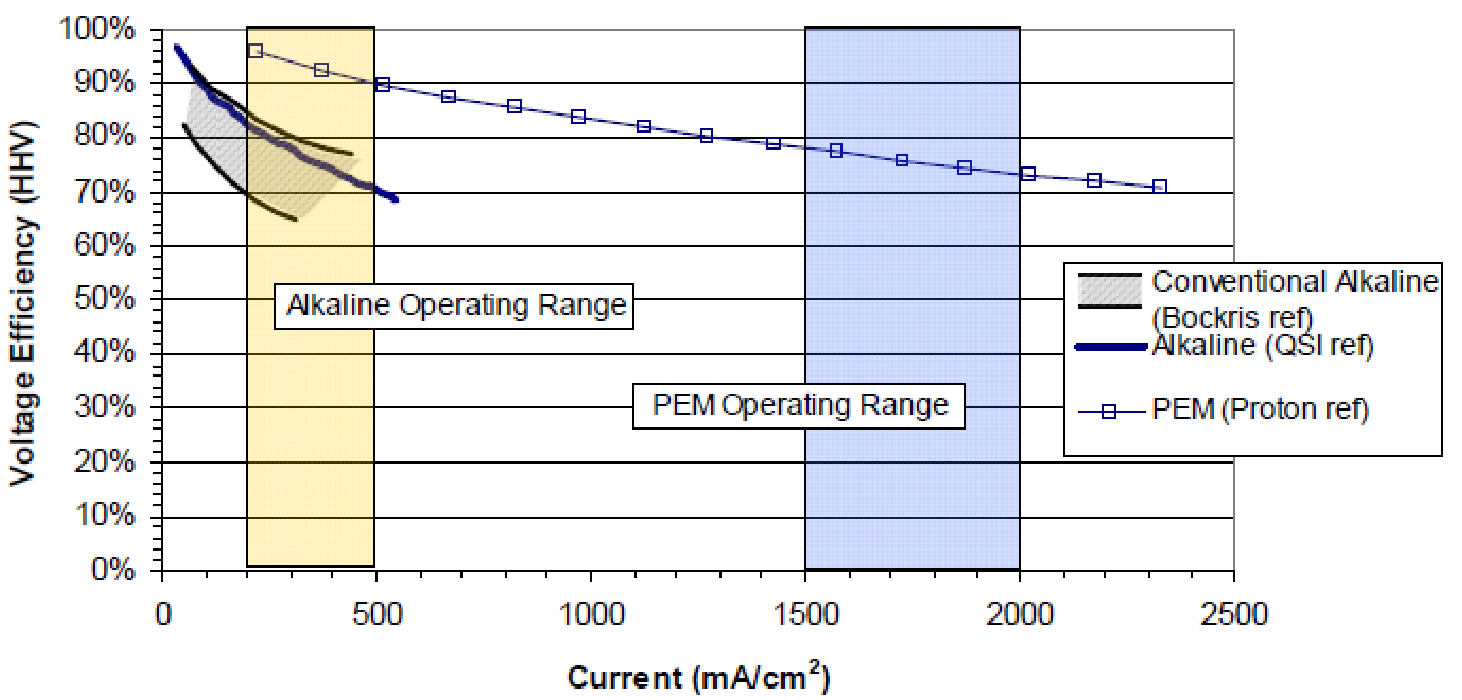
\includegraphics[width=0.7\linewidth]{content/Grafiken/Ely-Efficiency}
	\caption[Elektrolyseur Spannungseffizienz]{Elektrolyseur Spannungseffizienz \cite{NOWH2}}
	\label{fig:ely-efficiency}
\end{figure}


\section{Stromrichter}
\label{sec:Stromrichter}
Allgemein kann man jede Schaltung die zur Strom- und Spannungsversorgung dient als Stromrichter bezeichnen, dabei wird unterschieden zwischen Wechsel- und Gleichspannungsvarianten. Außerdem kann bei Netzanwendungen in gesteuerte, Netz-gesteuerte und ungesteuerte unterschieden werden, sowie die Umsetzung einer \gls{PFC} betrachtet werden. 
		\subsection{Gleichrichter}
		Ein Gleichrichter wird verwendet, um aus einer Wechselspannung eine Gleichspannung zu erzeugen. Die einfachste Form ist der Diodengleichrichter, dieser kann für einphasige Wechselspannung durch eine einzelne Diode realisiert werden. Jedoch würde so nur die halbe Periode des Sinus am Ausgang zur Verfügung stehen, da die Diode nur während der positiven Halbwelle Leitet. Dies lässt sich durch die Ergänzung zum Brückengleichrichter mit vier und für dreiphasige Anwendungen mit sechs Dioden ausgestattet ist.\\
		Anhand des Diodengleichrichters wird schnell klar, dass eine solche Schaltung nur bedingt für einen gewünschten Stromverlauf sorgt. In Abbildung \ref{B6DiodRect} sind Netzspannung und Strom dargestellt, der Stromverlauf zeigt Starke Sprünge und der gewünschte Sinusförmige Verlauf ist nur schwer erkennbar. Außerdem lässt sich mit dieser Schaltung die Ausgangsspannung sowie der Strom nicht variieren.
		\begin{figure}[H]
			\centering
			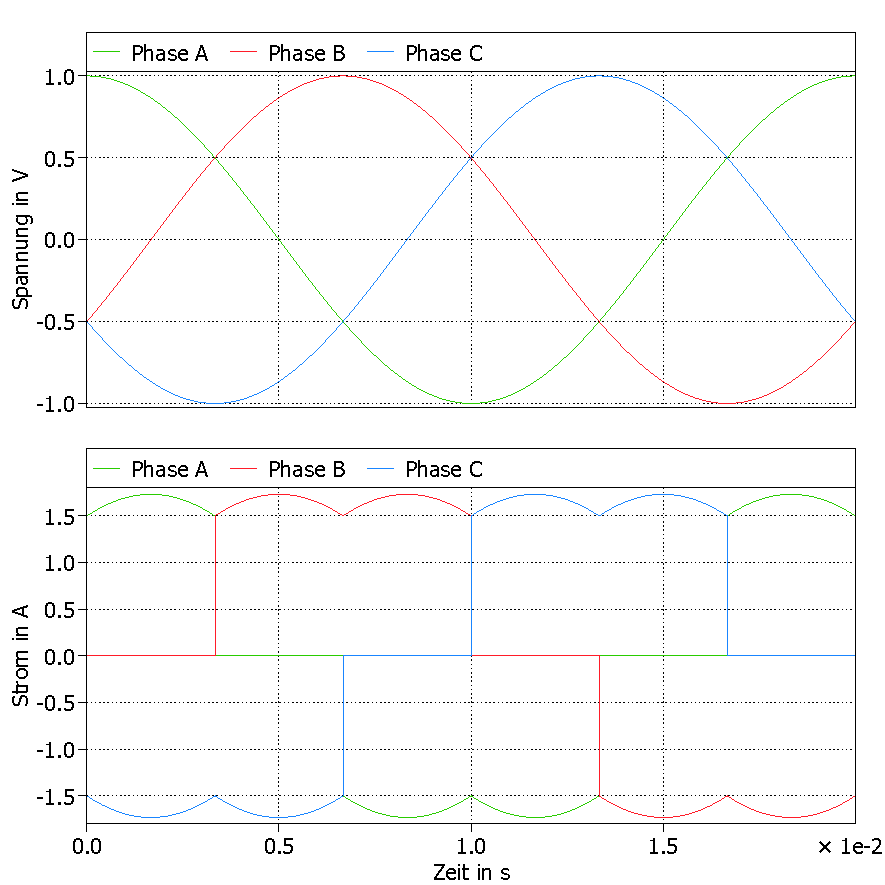
\includegraphics[width=0.7\linewidth]{content/Grafiken/B6-Diodengleichrichter-Eingangsverlauf}
			\caption{Strom und Spannungsverlauf am B6 Diodengleichrichter}
			\label{B6DiodRect}
		\end{figure}
		
		Für Elektrolyseanlagen mit mehreren Megawatt Leistung müssen Zwangsweise Leistungshalbleiter parallelisiert werden, da bei Spannungen bis 1000 V die Ströme für einzelne Halbleiter zu hoch sind. Außerdem bietet die Parallelisierung durch Interleaving und Phasenverschiebung deutliche Vorteile für die Verzerrung und damit Filterung. 
		
		\subsection{DC-DC Wandler}
		Der Hoch- und Tiefsetzsteller sind essenzielle Topologien und bestehen im wesentlichen aus einer Diode, einem Schalter und einer Induktivität. 
			
		\subsection{Power Factor Correction}
			Die \gls{PFC} ist eine nötige Maßnahme um den Blindleistungsanteil im Netz zu reduzieren 
			The front-end circuit concept of the H3R system was first introduced in late 90s by Jantsch and Verhoeve,

In gängigen Gleichrichtersystemen werden getrennte Einheiten bestehend aus einer dreiphasigen PFC-Gleichrichterschaltung und einem Gleichspannungswandler (DC/DC-Buck-Wandler) eingesetzt, um die Anforderungen zu erfüllen. Die Regelung der beiden Wandlerstufen ist in der Regel entkoppelt, wobei der Gleichrichter sinusförmige Netzströme zieht und der nachfolgende DC/DC-Wandler die Spannung auf den erforderlichen Ausgang anpasst. Auf der Suche nach kompakten und leichten Systemen sind hohe Schaltfrequenzen notwendig, was jedoch zu erhöhten Schaltverlusten und verringerter Wandlereffizienz führen kann. Um dies zu adressieren, werden fortgeschrittene Modulationstechniken wie Einfügen der dritten harmonischen und Raumzeigermodulation möglich. Alternativ kann auch Diskontinuierliche Pulsweitenmodulation (DPWM) als Methode zur Reduzierung der Schaltverluste in dreiphasigen PFC-Gleichrichtern verwendet werden, um sinusförmige Eingangsströme und eine konstante Gleichspannung sicherzustellen. Im Gegensatz dazu müssen Einstufen-Wandlersysteme beide Anforderungen gleichzeitig erfüllen, während Zweistufen-Systeme trotz niederfrequenter Spannungsschwankungen im Zwischengleichspannungsnetz eine konstante Ausgangsspannung sicherstellen können.			
			
\section{IAF Rectifier}
Der \gls{IAF} Gleichrichter wurde erstmals vorgestellt in \cite{IAFfirst} im Jahr 1997 . Dieser besteht für den Hauptleistungspfad aus einem Diodengleichrichter, um sinusförmige Ströme in allen drei Phasen einzuprägen wird dieser durch ein Netzwerk aus bidirektional Sperrenden Leistungshalbleitern ergänzt, welche einen Strom in den Gleichrichter einprägen. Durch die Integration des Filters in den Leistungspfad, kann die Kompensation effizienter funktionieren. Aufgrund des ungesteuerten Diodengleichrichters wird jedoch eine anschließende Spannungsregelung durch einen Tiefsetzsteller benötigt.

\section{1/3 PWM PFC Rectifier}
Bei dieser Topologie handelt es sich um eine gängige Schaltung, welche durch ein neuartiges Modulationsverfahren unter Verwendung von Induktivitäten auf der Netzseite eine Reduzierung der Schaltverluste bewirkt und Blindleistung ermöglicht. Das Verfahren wurde ausführlich von Menzi, Bortis und Kolar beschrieben \cite{13PWMPFC}.



\section{Leistungshalbleiter}

\section{Induktivitäten}

\section{Simulationssoftware}
Zur Bewertung und Betrachtung der Umsetzbarkeit, der Topologien ist es nötig diese in einer Umfassenden Simulation zu betrachten. Dies ermöglicht es die Funktionalität und den Einfluss der Parameter im direkten Zusammenspiel zu untersuchen. Insbesondere das Verhalten für Systemdienstleistungen, wie Phasenverschiebung und die dadurch beeinflusste Verteilung der Verlustleistungen sollen als Entscheidungsgrundlage dienen. 

	\subsection{PLECS}
	Die Software \gls{PLECS} aus dem Haus PLEXIM wird als Integration in MATLAB mit Simulink verwendet.  
\chapter{Anforderungen}
\label{chap:Anforderungen}

\section {Stromnetz}
In Deutschland sind die Vorgaben für den Anschluss von Anlagen an das Stromnetz durch den \gls{VDE} definiert. Je nach Anschlussleistung, Standort und Betriebsverhalten, wird eine unterschiedliche Netzspannungsklasse gewählt, welche geringfügig abweichende Anschlussrichtlinien besitzt. Aufgrund der Skalierbarkeit zu höheren Leistungsklassen und der erwartbar steigenden Anforderungen, wird sich für die Anforderungen der Hochspannung entschieden. Diese hat die Bezeichnung VDE-AR-N 4120 "Technische Regeln für den Anschluss von Kundenanlagen an das Hochspannungsnetz und deren Betrieb (TAR Hochspannung)" \cite{VDEARN4120}.
Hierzu zählt unter anderem die Anforderung an die Phasenverschiebung, bei Wirkleistungsbezug darf eine maximale Verschiebung von $cos(\phi)=0,95$ was einem Winkel von etwa 18 Grad entspricht auftreten vgl. Abb. \ref{fig:tar4120pq}. Jedoch kann der Netzbetreiber mit dem Anlagenbetreiber gesonderte Vereinbarungen treffen, dies ermöglicht es Netzdienstleistungen anzubieten. Dies führt zur Anforderung an die Topologie eine Phasenverschiebung von mindestens 18 Grad zu ermöglichen.\\
\begin{figure}[H]
	\centering
	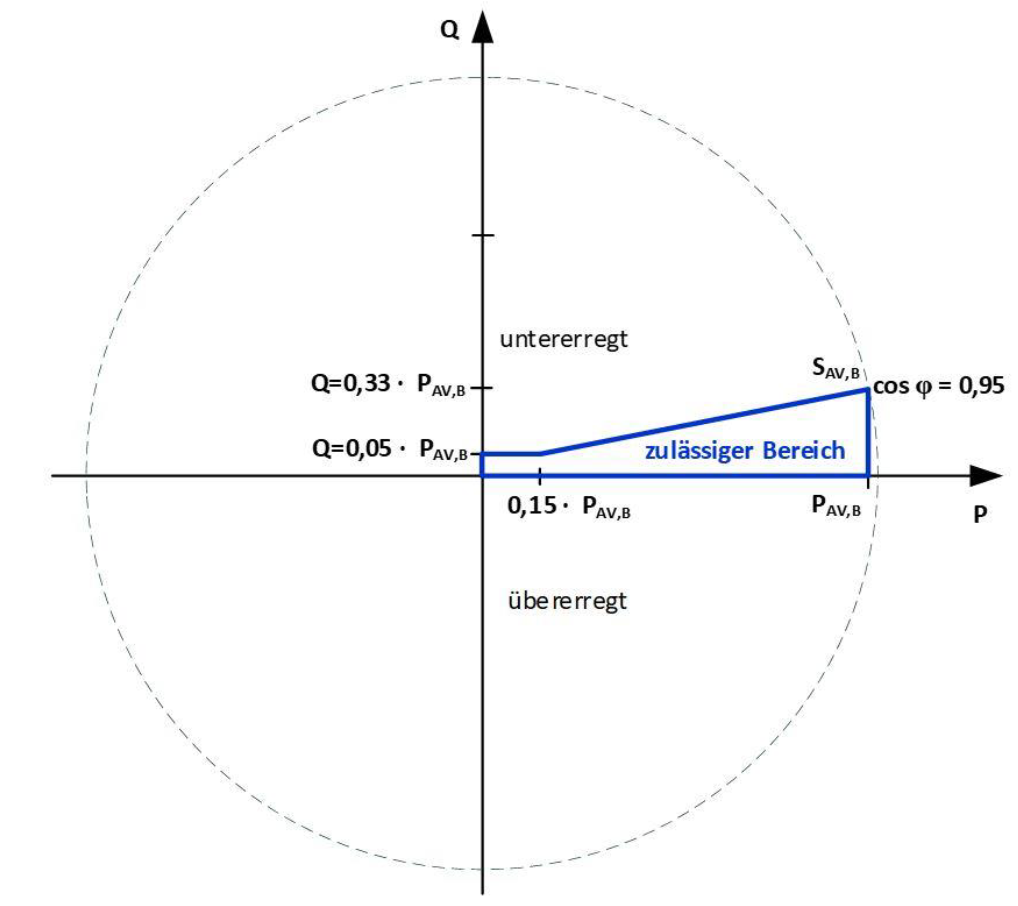
\includegraphics[width=0.6\linewidth]{content/Grafiken/TAR4120_PQ}
	\caption[Zulässiger Bereich des Verschiebungsfaktors cos $\phi$ bei Wirkleistungsbezug]{VDE TAR4120: Zulässiger Bereich des Verschiebungsfaktors \cite{VDEARN4120}}
	\label{fig:tar4120pq}
\end{figure}
Des weiteren sind zeitlich begrenzte Frequenz und Spannungsänderung die auftreten können definiert als quasistationärer Betrieb. Die Netzspannung kann im Bereich von +/- 15 Prozent Schwanken, sowie die Frequenz von 50 Hertz zwischen 47,5 und 51,5 variieren vgl. Abb \ref{fig:vde4120-Anforderungen} (a). Innerhalb dieses Bandes muss die Anlage im regulären Betrieb bleiben. Dabei wird ein Gradient von  <5 \%  im Spannungsband sowie <0,5 \% pro Minute im Frequenzband vorausgesetzt. \\
Im Fehlerfall durch Blitzeinschlag oder Kurzschluss, muss die Anlage kurzzeitig deutlich stärkere Spannungsschwankungen mit machen. Diese Anforderung wird als \gls{FRT} bezeichnet und kann für bis zu 100 Millisekunden die Spannung um 25 Prozent erhöhen vgl. Abb. \ref{fig:vde4120-Anforderungen} (b). Aufgrund eines Kurzschluss kann die Spannung auf 15 Prozent der eigentlichen Netzspannung abfallen. Dies stellt für Verbraucheranlagen eine große Herausforderung dar, da die zu betreibenden Systeme meist eine minimal Spannung benötigen.

\begin{figure}[H]
\centering
\subfloat[][]{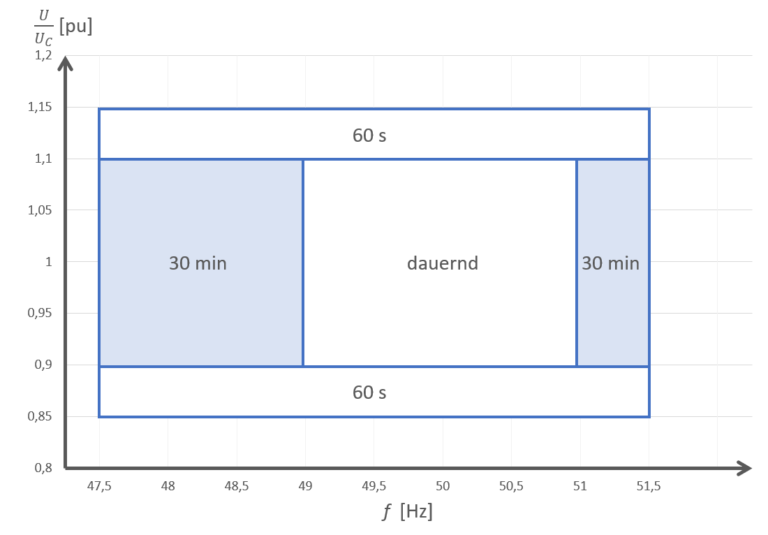
\includegraphics[width=0.7\linewidth]{content/Grafiken/VDE4120-quasistationarerbetrieb}}%
%\caption[Mindestanforderungen an den quasistationären Betrieb von Erzeugungsanlagen \cite{VDEARN4120]{Quasistationärer Betrieb}}

\qquad
\subfloat[][]{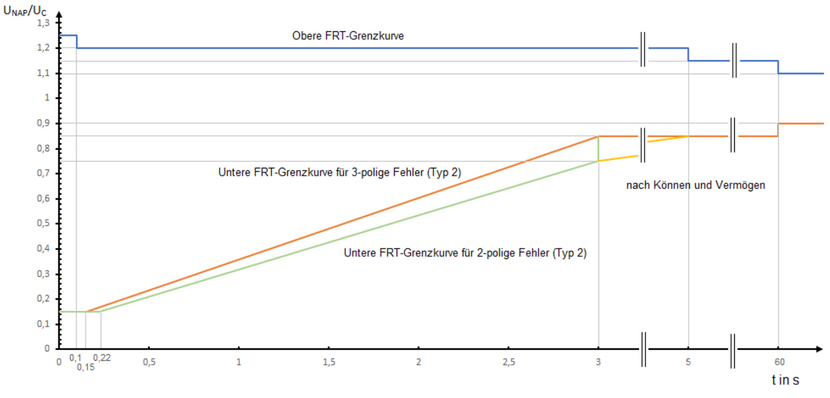
\includegraphics[width=0.7\linewidth]{content/Grafiken/Grenzkurve}}%

\caption[quasistationären Betrieb (a) und \gls{FRT} (b)]{Mindestanforderungen an den quasistationären Betrieb (a) und \gls{FRT} (b)}
\label{fig:vde4120-Anforderungen}
\end{figure}




\subsection{Systemanforderungen}


\subsection{Überspannungsschutz}

\section{Elektrolyseur}
Zur Elektrolyse wird eine Gleichspannung benötigt welche aufgrund von Alterungsprozessen, innerhalb der Zellmembrane, mit der Zeit ansteigt \cite{HydrogenElectronicTopologies}. Außerdem wird zu Beginn der Elektrolyse eine niedrige Spannung benötigt um den Prozess zu starten. Daher wird ein Bandbreite von 0 bis einigen 100 Volt benötigt. Um die gewünschte Leistung umsetzen zu können ist es für die Wirtschaftlichkeit relevant den Strom möglichst zu reduzieren, woraus eine höhere Spannung resultiert. Dies wird durch den modularen Zellaufbau unterstützt der eine Flexible Systemspannung ermöglicht. \\
Um die Effizienz und Lebensdauer des 
\section{Zusammenfassung}
Die Anforderungen an den Gleichrichter sind in Tabelle \ref{tab:AnfZsm} zusammengefasst, für die Implementierung wird die Zukünftige Betrachtung als relevant betrachtet.\\
\begin{table}
\caption{ Anforderungen an den Gleichrichter heute und in Zukunft}

\begin{tabular}{c|c|c}
	
	& Aktuell & Zukünftig \\
	\hline
	Leistungsfaktor stationär & >0.95 & >0.99 \\
		\hline
	Leistungsfaktor als Systemdienstleistung & keine Angabe & +/- 30° \\
	\hline
	$THD_i$ & <5 \% & <5\% \\
	\hline
	Ausgangsstromrippel & <5 \% & <2 \% \\
	\hline
	Ausgangsspannung & < 1000 V & < 1500 V \\
	
	
	\label{tab:AnfZsm}
\end{tabular}
\end{table}
\section{Bewertungskriterien}
Die Kriterien zur finalen Auswahl der Topologie setzen sich aus der Erfüllung der Anforderungen zusammen sowie der Bewertung der Hardware. Die Grundlegenden Anforderungen aus Seiten des Stromnetzes und Elektrolyseur wurden bereits in der Vorauswahl berücksichtigt und können nun im Detail anhand von \gls{THD} und Rippelgrößen betrachtet werden. Die Quantifizierung der Hardware wird zum einen anhand der Verlustleistung in den Halbleitern, welche indirekt auch den Kühlungsaufwand repliziert, zum anderen durch die Größe und den Aufwand für die Komponenten berücksichtigt.  
\chapter{Vorauswahl}
Um die möglichen Optionen einzugrenzen, werden im Folgenden die Topologien aufgelistet und die Auswahl anhand einfacher Kriterien eingegrenzt. Einen guten Überblick über Schaltungen für dreiphasige Gleichrichter mit Blindleistungskompensation geben die Präsentationen von Dominik Bortis et al. \cite{Advanced3PhPFC} und Johann W. Kolar \cite{Essenceof3pKolar}. Dabei handelt es sich um Systeme mit aktiver Leistungsfaktorkorrektur. Aufgrund der gewünschten Systemdienstleistungen, wie z.~B. Blindleistungsbereitstellung, sind Systeme mit hybrider Kompensation nicht ausreichend.

\section{Mögliche Topologien}
Die als Vergleichstopologie verwendete ist der bereits im Abschnitt \ref{sec:Rec} vorgestellte dreiphasige Diodengleichrichter. Die anderen Topologien sind nachfolgend aufgeführt.
	\subsection{6-Switch Boost PFC Rectifier}
				Bei der ersten Topologie wurden im Prinzip beim Diodengleichrichter die Dioden durch Schalter ersetzt, siehe Abbildung \ref{fig:sixswitchboost} Dies ermöglicht im Zusammenspiel mit den Eingangsimpedanzen ein Boost-Verhalten und die Modulation der Eingangsströme über verschiedene \gls{PWM}-Verfahren zum gewünschten sinusförmigen Eingangsstrom.
			\begin{figure} 
				\centering
				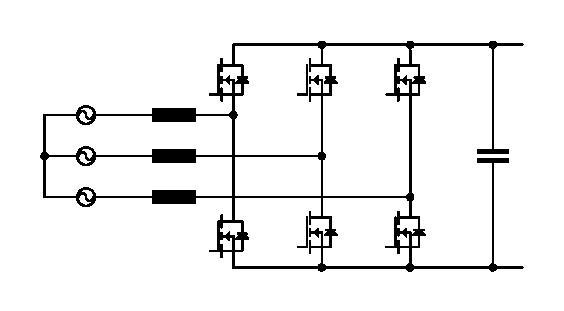
\includegraphics[width=1\linewidth]{content/Grafiken/SixSwitchBoost}
				\caption{Six Switch Boost PFC Rectifier}
				\label{fig:sixswitchboost}
			\end{figure}
		
	\subsection{6-Switch Buck PFC Rectifier}
		\label{sec:6switchBuck}
		Durch das Verschieben der Drossel auf die Ausgangsseite entsteht aus dem 6-Switch Boost eine Tiefstellende Topologie. Allerdings wird ein sperrendes Verhalten in beide Richtungen benötigt, um die Ausgangsspannung und den Eingangsstrom in die gewünschte Form zu bringen. Durch die Schalter wird der Tiefsetzende Strompfad ermöglicht. Aus diesem Grund werden die Schalter durch Dioden ergänzt, wie in Abbildung \ref{fig:sixswitchbuck} dargestellt.  
		
		\begin{figure}
			\centering
			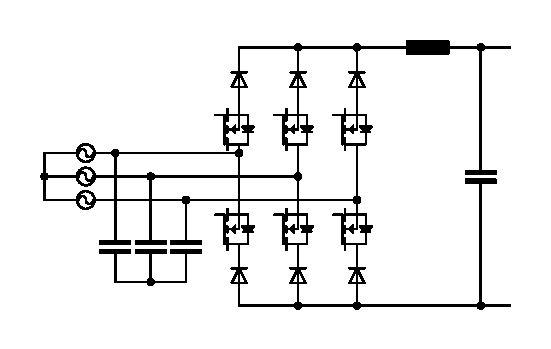
\includegraphics[width=1\linewidth]{content/Grafiken/SixSwitchBuck}
			\caption{Six Switch Buck PFC Rectifier}
			\label{fig:sixswitchbuck}
		\end{figure}
		
		\subsection{Trident Rectifier}
		Diese Topologie basiert auf dem 6-Switch Boost Rectifier. An jeder Phasenhalbbrücke ist ein eigener Tiefsetzsteller angeschlossen. Dadurch besitzt jede Phase einen unabhängigen, identischen parallelen Aufbau zwischen AC- und DC-Pfad (siehe Abbildung \ref{fig:trident}). Dies ermöglicht kontinuierliche Ein- und Ausgangsströme und durch die Wahl des Hoch- oder Tiefsetzenden Strompfades verringern sich die Schaltverluste.
		\begin{figure}
			\centering
			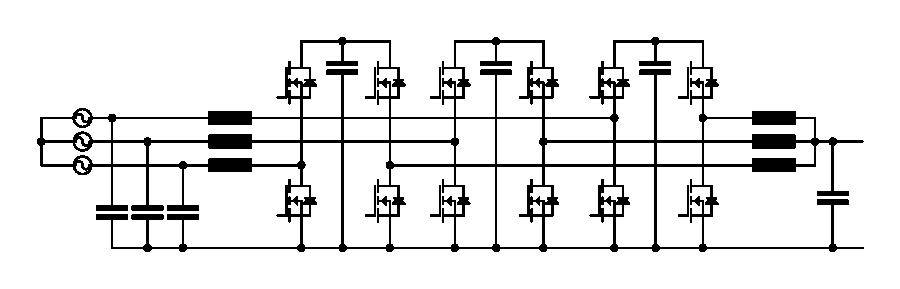
\includegraphics[width=1\linewidth]{content/Grafiken/Trident}
			\caption{Trident Rectifier}
			\label{fig:trident}
		\end{figure}
		
		\subsection{Vienna Rectifier}
		Hierbei handelt es sich ebenfalls um eine hochsetzstellende Topologie. Sie besteht aus einem Diodengleichrichter mit Eingangsinduktivitäten und wird durch einen \gls{IVS} ergänzt, an dem Kapazitäten zur Erzeugung der Ausgangsspannung zugeschaltet werden können. Siehe Abbildung \ref{fig:vienna}. Durch diese 3-Level Struktur kann eine bessere Form des Eingangsstroms erreicht werden als bei der 2-Level 6-Switch Boost PFC Topologie. Durch das weitere Spannungslevel, kann in feineren Stufen geschaltet und somit präziser die gewünschte Stromform eingestellt werden. Außerdem kann aus gleichem Grund die Induktivität kleiner ausfallen.
		\begin{figure}
			\centering
			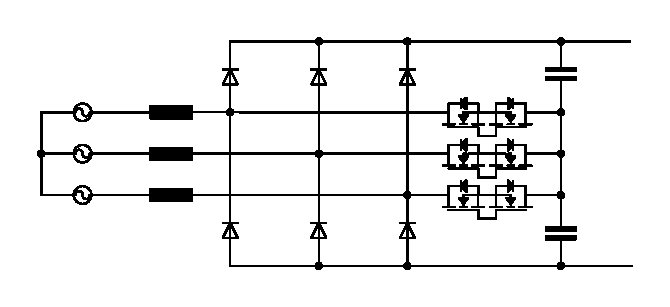
\includegraphics[width=1\linewidth]{content/Grafiken/Vienna}
			\caption{Vienna Rectifier}
			\label{fig:vienna}
		\end{figure}
	
	\subsection{Swiss Rectifier}
		Diese Topologie integriert den Tiefsetzsteller in die Schaltung des \gls{IAF}, siehe Abschnitt \ref{sec:IAF}. Dazu wird die Induktivität im IVS-Pfad mit der des Tiefsetzstellers kombiniert und der Schalter des Tiefsetzstellers durch eine Diode ersetzt. Die Schaltung ist in Abbildung \ref{fig:swiss} zu finden. Durch die Einsparung des Schalters kann die Effizienz gesteigert werden.
		\begin{figure}
			\centering
			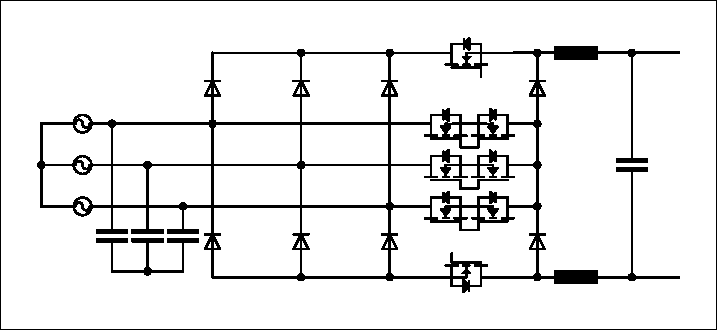
\includegraphics[width=1\linewidth]{content/Grafiken/Swiss}
			\caption{Swiss Rectifier}
			\label{fig:swiss}
		\end{figure}
		
	\subsection{2/3 PWM Buck \& Boost Current Source Rectifier} \label{sec:2/3BuckBoost}
		Um einen größeren Bereich an Ausgangsspannungen abdecken zu können, wird der 6-Switch Buck mit Bidirektionalen Schaltern und durch einen Hochsetzsteller am Ausgang erweitert. Dies zeigt die Abbildung \ref{fig:23pwmbuckboost}. 
		\begin{figure}
			\centering
			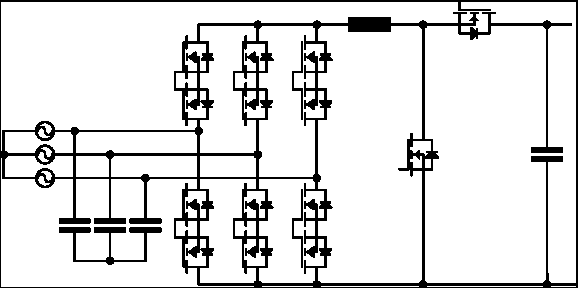
\includegraphics[width=1\linewidth]{content/Grafiken/23PWMBuckBoost}
			\caption{2/3 PWM Buck \& Boost Current Source Rectifier}
			\label{fig:23pwmbuckboost}
		\end{figure}
	
		
	\subsection{Y-Rectifier}
		Anstelle der Topologie aus \ref{sec:2/3BuckBoost} mit Hoch- und Tiefsetzsteller wird hier die umgekehrte Variante mit Tief- und Hochsetzsteller verwendet. Dies ermöglicht kontinuierliche Ein- und Ausgangsspannungen. Außerdem sinken die Schaltverluste, da jeweils nur der Hoch- oder Tiefsetzende Pfad geschaltet wird. Die Schaltung ist in Abbildung \ref{fig:y-rectifier} gezeigt.
		
	
		\begin{figure}
			\centering
			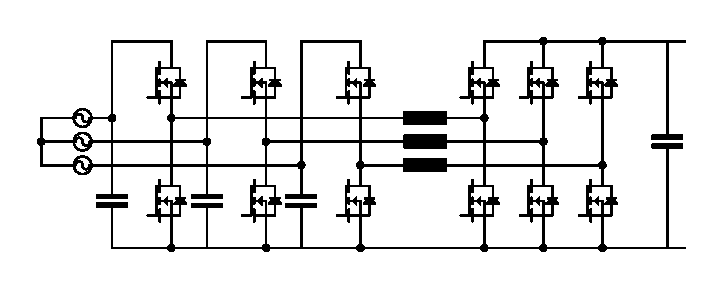
\includegraphics[width=1\linewidth]{content/Grafiken/Y-Rectifier}
			\caption{Y Rectifier}
			\label{fig:y-rectifier}
		\end{figure}
	
	\subsection{3-Level Neutral Point Clamped (NPC)}
		Die 3L-\gls{NPC}-Schaltung ist eine langjährig entwickelte Topologie, die durch verschiedene Ansteuerverfahren unterschiedliche Eigenschaften erzeugt. Unter anderem kann die Reduzierung der Oberschwingungen im Netzstrom und der Rechenaufwand durch optimierte Ansteuerungen verbessert werden \cite{NPC}. Die Schaltung benötigt insgesamt 12 Schalter und 6 Dioden sowie eine dreiphasige Drossel. Der vereinfachte Aufbau der Schaltung ist in Abbildung \ref{fig:3l-npc} dargestellt.
		\begin{figure}
			\centering
			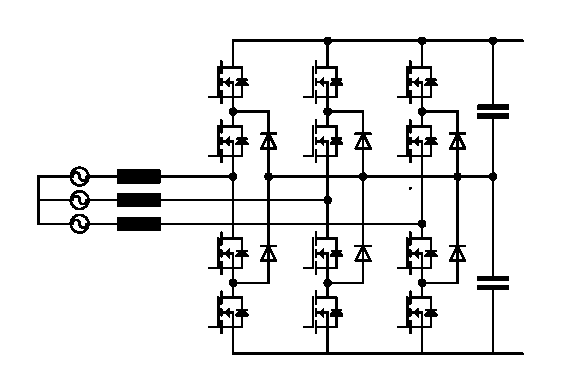
\includegraphics[width=1\linewidth]{content/Grafiken/3L-NPC}
			\caption{3-Level Neutral Point Clamped}
			\label{fig:3l-npc}
		\end{figure}

	\subsection{3-Level Active Neutral Point Clamped (ANPC)}
		Bei der \gls{ANPC}-Schaltung werden die Dioden der \gls{NPC}-Schaltung durch Schalter ersetzt, um den Sternpunkt kontrollieren zu können, siehe Abbildung \ref{fig:anpc}. Auch hier gibt es verschiedene \gls{PWM}-Strategien, die unterschiedliche Schwerpunkte setzen, außerdem ist die Verteilung der Verlustleistung in den Halbleitern nicht trivial \cite{ANPC}.
	
		\begin{figure}
			\centering
			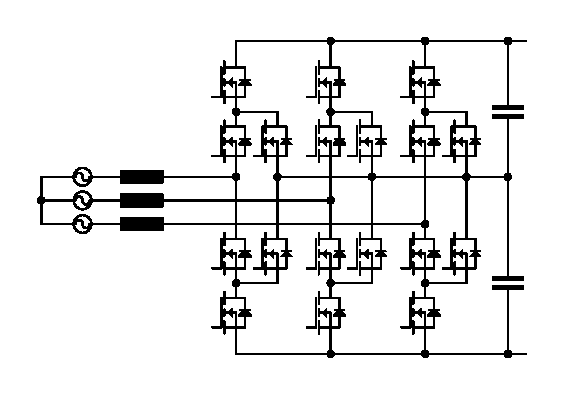
\includegraphics[width=0.9\linewidth]{content/Grafiken/ANPC}
			\caption{3-Level ANPC}
			\label{fig:anpc}
		\end{figure}
	
	
	\subsection{Three-Level Flying Capacitor (FC) Boost-Type Rectifier System}
		Diese Topologie benötigt Kondensatoren für jede Phase, die ein größeres Volumen besitzen, benötigt jedoch weniger Schalter für die drei Level. Die Schaltung ist in Abbildung \ref{fig:3l-fc-boost} dargestellt und besitzt ein hochstellendes Verhalten.
		\begin{figure}
			\centering
			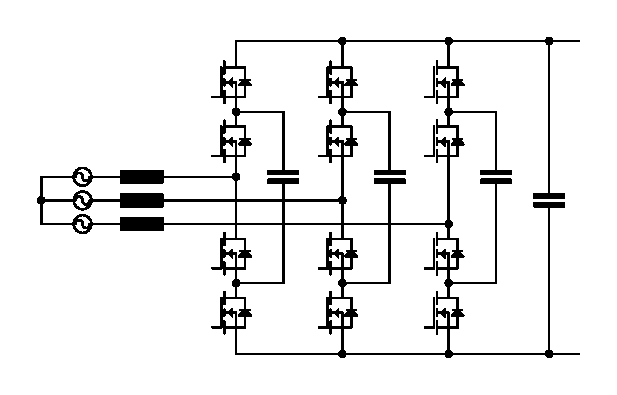
\includegraphics[width=1\linewidth]{content/Grafiken/3L-FC-Boost}
			\caption{Three Level Flying Capacitor Boost-Type}
			\label{fig:3l-fc-boost}
		\end{figure}
	
	
	\subsection{Three-Level Flying Capacitor (FC + Tiefsetzsteller)}
		Um den gewünschten niedrigen Ausgangsspannungsbereich generieren zu können, wird die zuvor beschriebene FC-Topologie durch einen Tiefsetzsteller ergänzt. Dadurch erhöht sich die Anzahl der benötigten Schalter von 12 auf 14.
		\begin{figure}
			\centering
			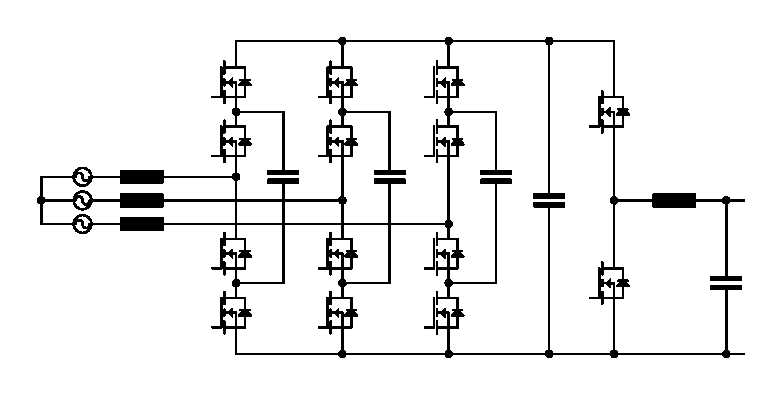
\includegraphics[width=1\linewidth]{content/Grafiken/3L-FC-Boost+Buck}
			\caption{3L FC + Tiefsetzsteller}
			\label{fig:3l-fc-boostbuck}
		\end{figure}

\section{Auswahl der Topologien}
Zur Eingrenzung des Lösungsraums wird zunächst eine Auflistung der möglichen Schaltungstopologien zum Anschluss an das dreiphasige Stromnetz erstellt, vergleiche Tabelle \ref{tab:vorauswahl}. Die 15 aufgelisteten Topologien, beginnend mit dem in Abbildung \ref{fig:B6DiodRect} dargestellten Diodengleichrichter, werden anhand der benötigten Induktivitäten, Dioden, Schalter und Stufen, sowie der Funktionen hoch- bzw. tiefstellend bewertet.\\
Aufgrund ihres simpleren Aufbaus sind Dioden günstiger als Leistungsschalter und fallen daher nicht so stark ins Gewicht. \\
Daher ist der Swiss Rectifier trotz seiner 8 Dioden aber lediglich benötigter 8 Schalter von Interesse. Reine hochsetzende (Boost) Topologien kommen für die Anwendung nicht infrage, da eine niedrige Spannung als Anforderung gestellt wird um den Elektrolyseur hochzufahren. \\
Die Tabelle \ref{tab:vorauswahl} zeigt, dass sich die vier Topologien, die grün hervorgehoben sind, für eine engere Betrachtung eignen, da sie im Vergleich zu anderen Topologien weniger Induktivitäten und Halbleiter benötigen. Die Anzahl der Halbleiter beeinflusst die Kosten und Effizienz der Schaltung und spielen daher eine essentielle Rolle. Anhand der Anzahl an Induktivitäten im Hauptstrompfad wird der Einfluss dieser verglichen. \\
Aufgrund der Komplexität der Schaltungen und benötigten Regelungen werden in dieser Arbeit der \gls{IAF} und \gls{B6PFC} betrachtet und die Ergebnisse für eine finale Bewertung aufbereitet. Die beiden anderen Topologien, 6-Switch Buck und Swiss Rectifier, werden in  der Arbeit von Steffen Isfort betrachtet.

\begin{table}
	\caption{Topologievergleich zur Vorauswahl}
	\label{tab:vorauswahl}
\begin{tabular}{|>{\centering\arraybackslash}p{3cm}| >{\centering\arraybackslash}m{2cm}|>{\centering\arraybackslash}m{2cm} | >{\centering\arraybackslash}m{2cm}|>{\centering\arraybackslash}m{2cm} |>{\centering\arraybackslash}m{2cm} |}
	\hline
	& Induktivitäten & Dioden & Schalter & Buck/Boost & Stufen \\
	\hline
	3-ΦDiode Bridge Rectifier & \cellcolor{yellow!25}3 &\cellcolor{red!25}6 &\cellcolor{green!25} 0 & \cellcolor{red!25}- & \cellcolor{green!25}1 \\
	\hline
	6-Switch Boost PFC Rectifier & \cellcolor{yellow!25}3 &\cellcolor{green!25} 0 & \cellcolor{green!25}6 & \cellcolor{red!25}Boost & \cellcolor{green!25}1 \\
	\hline
	Vienna Rectifier & \cellcolor{yellow!25}3 &\cellcolor{red!25}6 & \cellcolor{green!25}6 & \cellcolor{red!25}Boost & \cellcolor{green!25}1 \\
	\hline
	\cellcolor{green!10}6-Switch Buck PFC Rectifier & \cellcolor{green!25}1 &\cellcolor{red!25}6 &\cellcolor{green!25} 6 & \cellcolor{green!25}Buck & \cellcolor{green!25}1 \\
	\hline
	\cellcolor{green!10} \gls{IAF} & \cellcolor{green!25} 2 &\cellcolor{red!25}6 & \cellcolor{yellow!25}10 & \cellcolor{green!25}Buck & \cellcolor{red!25}2 \\
	\hline
	\cellcolor{green!10}Swiss Rectifier & \cellcolor{green!25}1 &\cellcolor{red!25}8 &\cellcolor{green!25} 8 & \cellcolor{green!25} Buck & \cellcolor{red!25}2 \\
	\hline
	\cellcolor{green!10} \gls{B6PFC} &\cellcolor{yellow!25}4 & \cellcolor{green!25} 0 &\cellcolor{green!25} 8 &\cellcolor{green!25} Boost/Buck & \cellcolor{red!25}2 \\
	\hline
	2/3 PWM Buck \& Boost Current Source Rectifier & \cellcolor{green!25} 1 & \cellcolor{green!25}0 & \cellcolor{yellow!25}14 & \cellcolor{green!25}Buck/Boost & \cellcolor{red!25}2 \\
	\hline
	Trident Rectifier & \cellcolor{red!25}6 &\cellcolor{green!25}0 & \cellcolor{yellow!25}12 & \cellcolor{green!25}Buck/Boost & \cellcolor{red!25}2 \\
	\hline
	Y-Rectifier & \cellcolor{yellow!25}3 &\cellcolor{green!25}0 & \cellcolor{yellow!25}12 &\cellcolor{green!25} Buck/Boost & \cellcolor{red!25}2 \\
	\hline
	3-Level Neutral Point Clamped & \cellcolor{yellow!25}3 &\cellcolor{red!25}6 & \cellcolor{yellow!25}12 & \cellcolor{red!25}Boost & \cellcolor{green!25}1 \\
	\hline
	3-Level Active Neutral Point Clamped  & \cellcolor{yellow!25}3 & \cellcolor{green!25}0 & \cellcolor{red!25}18 & \cellcolor{red!25}Boost & \cellcolor{green!25}1 \\
	\hline
	3-Level Active Neutral Point Clamped + Tiefsetzsteller & \cellcolor{yellow!25}4 &\cellcolor{green!25} 0 & \cellcolor{red!25}20 & \cellcolor{green!25}Boost/Buck & \cellcolor{red!25}2 \\
	\hline
	Three-Level Flying Capacitor (FC) Boost-Type Rectifier System & \cellcolor{yellow!25}3 & \cellcolor{green!25}0 & \cellcolor{yellow!25}12 & \cellcolor{red!25}Boost & \cellcolor{green!25}1 \\
	\hline
	Three-Level Flying Capacitor (FC + Tiefsetzsteller) & \cellcolor{yellow!25}4 &\cellcolor{green!25}0 & \cellcolor{yellow!25}14 &\cellcolor{green!25} Boost/Buck &\cellcolor{red!25} 2 \\
	\hline
\end{tabular}
\end{table}

\chapter{Simulation}


\section{Randbedingungen}

Die Regelung benötigt eine Erkennung des aktuellen Phasenwinkelabschnitts, diese ist implementiert nach \cite{InstituteofElectricalandElectronicsEngineers}.

\section{IAF}

\cite{IAF99}

\subsection{Auslegung der Induktivitäten }
\subsection{Regelung}

\subsection{Ergebnisse}


\section{B6 1/3 PFC Buck}
Die in Kapitel \ref{sec:GrundlagenB6} dargestellte Schaltung wird durch Halbbrücken Module des Typs FF2MR12W3M1H\_B11 von Infineon implementiert. Dabei handelt es sich um verbreitete 1200 \si{\volt} Module, sie besitzen einen nominellen Einschaltwiderstand von etwa 2 \si{\milli \ohm} und können Spitzenströme von bis zu 800 \si{\ampere} schalten \cite{IFAG-FF2}. Um die Ausgangsleistung auch bei geringerer Spannung bereitstellen zu können und ein späteres Interleaving zu ermöglichen werden für den Tiefsetzsteller zwei Halbbrücken vorgesehen.

\subsection{Auslegung der Induktivitäten }


\subsection{Regelung}
Die Regelung besteht aus einer Kaskadierten Struktur mit vier Stufen. Die erste ist die Ausgangsspannungsregelung, welche durch die Sollleistung und Netzspannung die gewünschte äquivalente Phasenimpedanz als Eingangsgröße für die Phasenstromregelung bildet.\\
In der dritten Stufe wird die Phase mit der mittleren Spannung ausgewählt und die Zwischenkreisspannung \gls{Upn} anhand der Phasenlage bestimmt. Die Zwischenkreisspannung resultiert als sechspulsige Gleichspannung und dient als Eingangsspannung für den Tiefsetzsteller. Die mittlere Phasenspannung wird als Referenz für den Tastgrad der entsprechenden Halbbrücke verwendet und prägt somit einen zur Spannung proportionalen Strom ein. Somit wird immer nur eine der drei Halbbrücken getaktet geschaltet, die anderen beiden sind wie bei einem Diodengleichrichter auf die jeweils positivste und negativste Spannung geschaltet.\\
Die vierte Stufe ist die des Tiefsetzstellers, mit Reglern für den Eingangsstrom sowie die Ausgangsspannung.

\begin{figure}
	\centering
	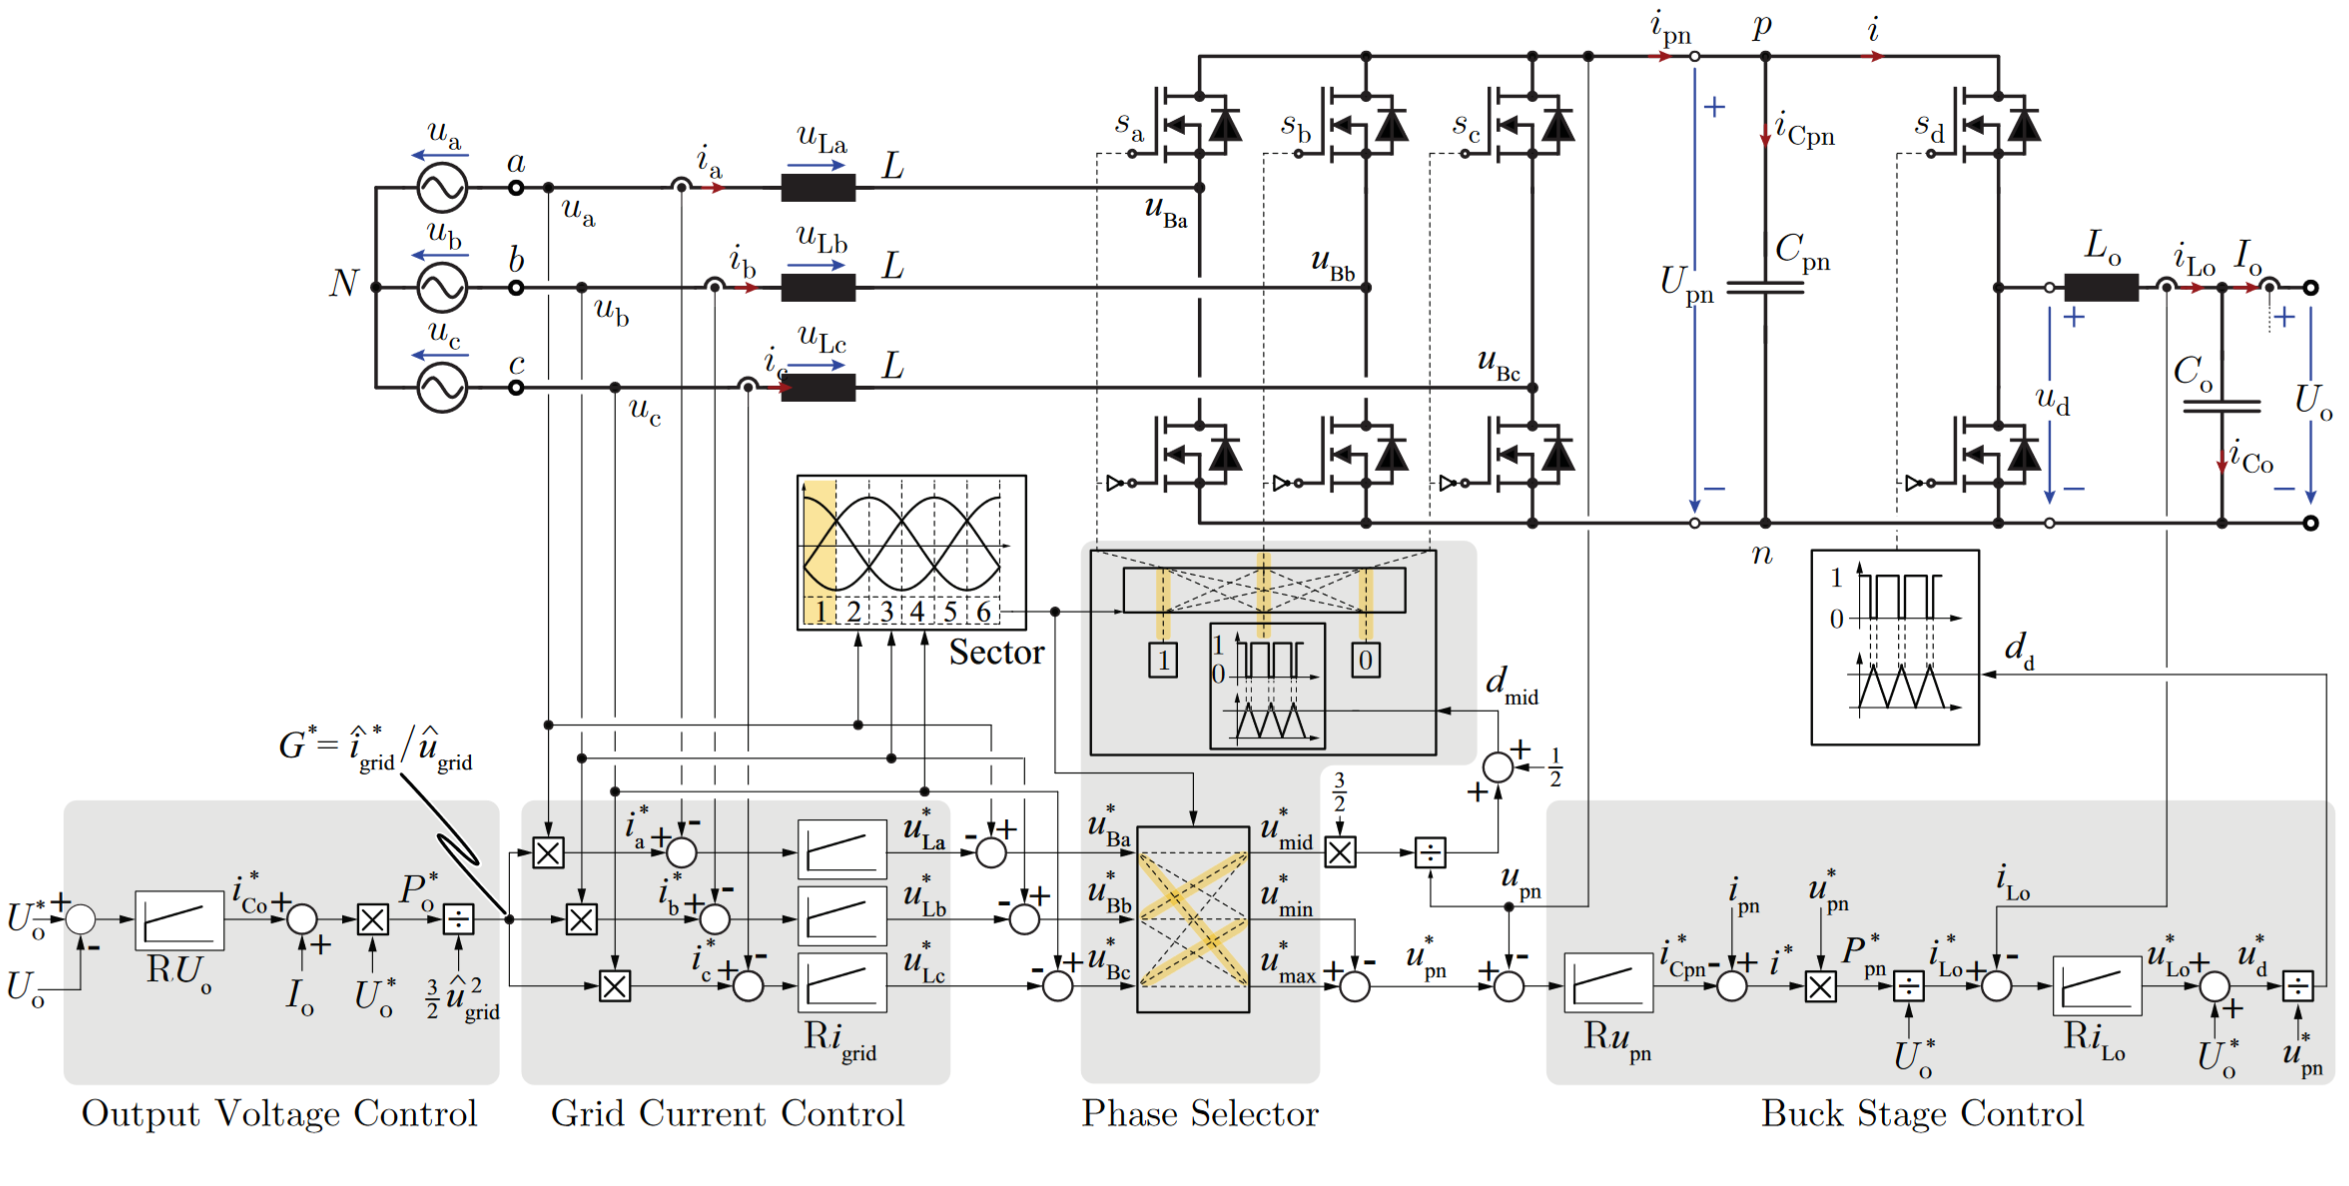
\includegraphics[width=0.9\linewidth]{content/Grafiken/B6-Control-orig}
	\caption[Regelung des \gls{B6PFC}]{Regelung des \gls{B6PFC} \cite{13PWMPFC}}
	\label{fig:b6-control-orig}
\end{figure}

\chapter{Auswertung}
Die Ergebnisse zur Gesamtbewertung finden sich in Tabelle \ref{tab:Auswertung}. Diese beinhaltet die Hardware, welche zum Großteil durch die Induktivitäten beeinflusst wird, sowie die Kapazitäten, Halbleiter und Treiber. Außerdem werden die Ergebnisse der Simulation durch die Verlustleistung der Halbleiter bewertet. Für die Simulation werden die in Tabelle \ref{tab:Betriebspara} aufgelisteten Betriebsparameter festgelegt. Die beiden Topologien werden für den Betriebspunkt mit 0° und 30° Phasenverschiebung verglichen, um den Einfluss der Systemdienstleistungen zu betrachten. Um einen Vergleich der Kategorien und eine Gesamtbewertung durchzuführen, werden die Einzelkategorien zwischen null und eins normiert und mit einem Gewichtungsfaktor die Summe über alle Kategorien gebildet. Aufgrund des großen Einflusses der Drosseln, werden diese mit 50 Prozent gewichtet. Die Kapazitäten stellen nur einen sehr geringen Einfluss auf das Gesamtsystem dar und werden daher nur mit fünf Prozent bewertet. Die restlichen 45 Prozent fallen auf die Halbleiter in Form der Chipfläche (über den \gls{RDSON}), Treiberanzahl und Verlustleistung ab. Je geringer die Punktzahl, desto besser ist die Bewertung. \\

	
\begin{table}
	\centering
\begin{tabular}{|c|c|}
	\hline
	Netzspannung \gls{Ull} & 617 \si{\volt} \\
	\hline
	Leistung & 200 kW bei $\phi$ 0° \\
	\hline
	Phasenverschiebung & 0 / 30 Grad \\
	\hline
	Kühlplattentemperatur & 100 °C \\
	\hline
	Schaltfrequenz & 20 kHz \\
	\hline
\end{tabular}
\caption{Auflistung der Simulationsbetriebsparameter}
\label{tab:Betriebspara}
\end{table}


\begin{table}
\begin{tabular}{|c|c|c|c|c|}
	\hline
	& Topologie & B6\_Buck & IAF & Gewichtung: \\
	\hline
	Induktivitäten [uH] & L1 Netzinduktivität & 136,0 & 1,0 &  \\
	\hline
	& L2 DC Induktivität & 136,0 & 136,0 &  \\
	\hline
	& Gespeicherte Energie & 7,8 & 7,8 &  \\
	\hline
	& L3 IAF IVS Induktivität & - & 302,2 &  \\
	\hline
	& Induktivität normiert: & 1,00 & 0,43 & 50\% \\
	\hline
	Kapazitäten [uF] & C1 Netzkapazität & - & 50,0 &  \\
	\hline
	& C2 Kondensator am Elektrolyseur & 1,0 & 1,0 &  \\
	\hline
	& C3 DC Zwischenkreis & 25,0 & 50,0 &  \\
	\hline
	& Kapazität normiert: & 0,26 & 1,00 & 5\% \\
	\hline
	Halbleiter & SiC 4 mOhm & 0,0 & 2,0 &  \\
	\hline
	& SiC 2 mOhm & 10,0 & 4,0 &  \\
	\hline
	& Vienna SiC 5 mOhm & 0,0 & 6,0 &  \\
	\hline
	& SiC normiert: & 1,00 & 0,64 & 15\% \\
	\hline
	& Vienna Diode & 0,0 & 6,0 &  \\
	\hline
	& Dioden normiert & 0,0 & 1,0 & 5\% \\
	\hline
	Treiber & Treiberanzahl & 8,0 & 7,0 &  \\
	\hline
	& Treiber normiert: & 1,00 & 0,88 & 5\% \\
	\hline
	Verluste [W] & Schaltverluste 30 Grad & 567,0 & 503,0 &  \\
	\hline
	& Leitverluste 30 Grad & 254,0 & 1311,0 &  \\
	\hline
	& 30 Grad normiert: & 75\% & 75\% &  \\
	\hline
	& Schaltverluste 0 Grad & 554,0 & 511,0 &  \\
	\hline
	& Leitverluste 0 Grad & 326,0 & 748,0 &  \\
	\hline
	& 0 Grad normiert: & 25\% & 25\% &  \\
	\hline
	& Verluste normiert: & 0,50 & 1,00 & 20\% \\
	\hline
	Gesamt &  &  0,813 & 0,654 & \\
	\hline
\end{tabular}
\caption{Auflistung der Simulationsergebnisse und Bewertung}
\label{tab:Auswertung}
\end{table}

\section{B6PFC}
Es zeigt sich, dass der \gls{B6PFC} deutliche Nachteile bei den Induktivitäten und somit den Hardwarekosten mit sich bringt.

\section{IAF}
Aufgrund der Anforderung an Blindleistungsbereitstellung hat die Topologie durch den \gls{IVS} einen Nachteil, da dieser sprunghafte Änderungen des Stromverlaufs verursacht. Diese starken Sprünge führen dazu, dass die \gls{THD} des Stroms deutlich verschlechtert wird. Somit kann der \gls{IAF} den Anforderungen nur sehr schwer gerecht werden, da weitere Filterstufen benötigt würden.
\chapter{Zusammenfassung \& Ausblick}
Die Ergebnisse in Tabelle \ref{tab:Auswertung} geben einen Überblick zum Vergleich der beiden Topologien, durch Gewichtung und Normierung können weitere Angaben ergänzt werden. Der \gls{IAF} schneidet in der Gesamtbewertung um etwa 0,2 Punkte besser ab, was hauptsächlich auf die optimierte Platzierung der Drossel zurückzuführen ist. In der Tabelle ist jedoch der Nachteil des \gls{IAF} bei Blindleistungsbereitstellung nicht abgebildet. Daher kann diese Topologie nach derzeitigem Kenntnisstand für diesen Anwendungsfall nicht empfohlen werden. Da der Strom in der Drossel zwischen den einzelnen Phasen umgeschaltet werden muss, kommt es zu starken Sprüngen im Eingangsstrom, was zu einem deutlich erhöhten Bedarf an Netzfiltern führt. Alternative Ansteuerverfahren zur Vermeidung der Sprünge durch die Phasenverschiebung können gegebenenfalls eine Optimierung bringen, konnten aber bisher nicht erfolgreich umgesetzt werden. Der \gls{B6PFC} bietet eine weit verbreitete Topologie, die bereits gut entwickelt ist. Aufgrund der großen Netzdrosseln hat sie jedoch höhere Anschaffungskosten und ein größeres Volumen. \\ 
Anhand der Bewertungsmatrix konnte die Finale Entscheidung über alle vier simulierten Topologien für den in Abschnitt \ref{sec:6switchBuck} dargestellten 6-Switch Buck Gleichrichter getroffen werden. Dieser bietet ähnlich wie der \gls{B6PFC} durch sechs Schalter Flexibilität für die Regelung des Eingangsstroms und optimiert gleichzeitig den Bedarf an Induktivitäten durch eine Ausgangsseitige Drossel. Jedoch bringt diese Schaltung einige Herausforderungen, da die Drossel einen konstanten Stromfluss benötigt und somit ein Stromzwischenkreis anstelle eines gängigeren Spannungszwischenkreises entsteht. Eine Tabelle der Bewertung über alle vier Topologien findet sich im Anhang, siehe Tabelle \ref{An:Entscheidungsmatrix}. Es ist zu sehen, dass der Six Switch Buck um 10 \% besser abschneidet als der \gls{IAF} und ebenfalls 5 \% besser als der Swiss Gleichrichter. \\
Für den Aufbau eines Demonstrators der endgültigen Topologie kann das Design der Halbleiter und Drosseln verwendet werden. Die Regler können als Basis verwendet werden, müssen aber um Sicherheitsfunktionen ergänzt werden und insbesondere muss die Stabilität des Gesamtsystems sichergestellt werden. Die Performance der gewählten Regler sowie die Stabilität über alle Betriebspunkte sollte betrachtet werden. Die Filter müssen entsprechend der benötigten Dämpfung im Bereich der Schaltfrequenzen für die Ein- und Ausgangsströme dimensioniert werden. Im System können Schwingungen durch das Schaltverhalten angeregt werden, insbesondere zwischen den Filterstufen und Hauptinduktivitäten. Darüber hinaus erfordert die Implementierung auf Hardware-Controllern weitere Optimierungen, um Abtastraten und Reglerverhalten zu definieren. Für \gls{SDL} und bei Netzfehlern wie Frequenzschwankungen sind entsprechende Stabilisierungsverhalten zu implementieren.\\

Wie im Kapitel \ref{sec:Grundlagen} erwähnt, sind die Halbleitermodelle ein essentieller Teil. Daher sollten sie optimiert und in die Simulation zurückgeführt werden. Die für diese Schaltung ausgewählten Halbleiter können beschafft und in einem Prüfstand vermessen werden. Der prinzipielle Versuchsaufbau ist in Abbildung \ref{fig:dpt} dargestellt. Er beinhaltet die Schaltzelle mit Mess- und Versorgungsgeräten sowie einer Sicherheitssteuerung. Die Messwerterfassung erfolgt über ein Oszilloskop, das automatisierte Messpunkte erfasst und speichert.  Anhand dieser Messdaten kann das Modell validiert, ergänzt und die Simulationsergebnisse optimiert werden. \\
\begin{figure}
	\centering
	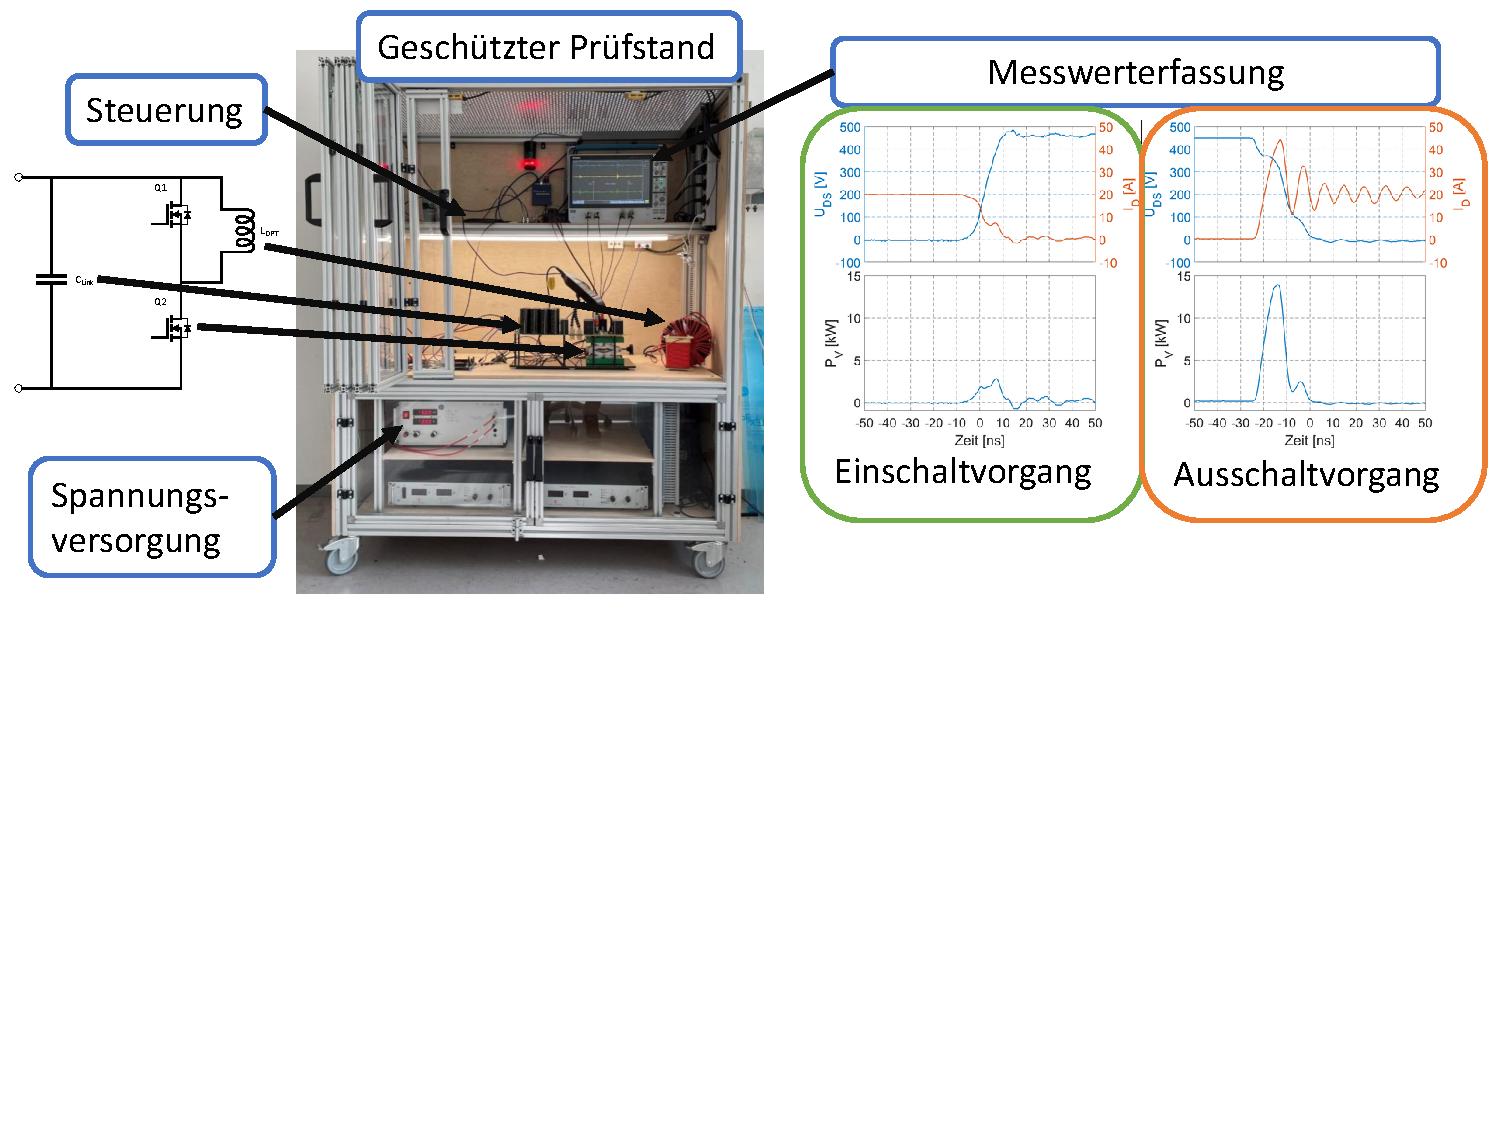
\includegraphics[width=0.95\linewidth]{content/Grafiken/DPT}
	\caption[Doppelpulstestprüfstand]{Doppelpulstestprüfstand}
	\label{fig:dpt}
\end{figure}
Ein weiterer Punkt ist der direkte Blitzeinschlag in das Stromnetz, der zu einer Spannungserhöhung führt. Entsprechende Funktionen und Spannungsgeneratoren können in die Simulation eingebaut werden, um die auftretenden Überspannungen an den Halbleitern zu ermitteln. Bei der Betrachtung fällt auf, dass bei beiden Topologien aufgrund des Aufbaus immer ein leitender Pfad über die Dioden gewährleistet ist. Die Energie kann somit im Zwischenkreiskondensator aufgenommen werden, wobei auf die Dimensionierung und die auftretenden Überspannungen an den Halbleitern zu achten ist. Der Strompfad über die Dioden in den Kondensator ist in Abbildung \ref{fig:iafsurge} dargestellt und ist identisch mit \gls{B6PFC}. \\
\begin{figure} [H]
	\centering
	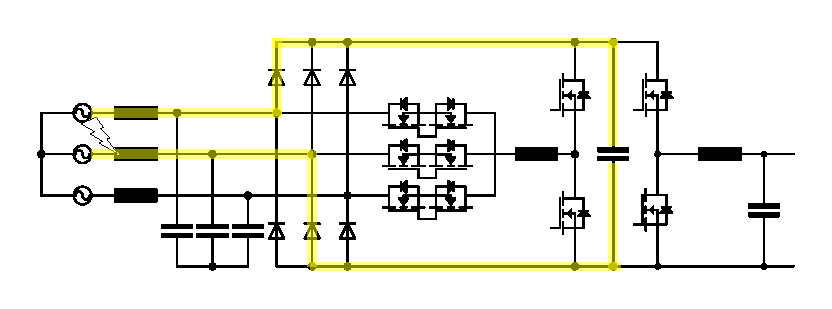
\includegraphics[width=0.95\linewidth]{content/Grafiken/IAF_surge}
	\caption{Strompfad im Fall eines Blitzeinschlag beim IAF}
	\label{fig:iafsurge}
\end{figure}

Die Schaltungen können außerdem durch Parallelbetrieb mit Interleaving am Ausgang oder bei entkoppelter Versorgung (durch getrennte Wicklungen am Netztransformator) als ausgangsseitige Reihenschaltung betrieben werden, um eine höhere Ausgangsspannung zu erzielen. Dabei sind weitere Regelungsparameter und Tests zur Betrachtung der Stabilität sowie des Auftretens unerwünschter Ausgleichsströme nötig. Um das Ziel einer Multimegawatt-Elektrolyseanlage zu erreichen, müssen mehrere Gleichrichter parallel betrieben werden. Daher ist die direkte Parallelisierung ein interessanter Aspekt für zukünftige Betrachtungen. Dies kann zunächst anhand von Simulationen durchgeführt werden, was den Rechenaufwand deutlich erhöht, um spätere Hardwaretests durchzuführen. Des weiteren kann der Hardwareaufbau in Kombination mit Echtzeitsystemen und Nachbildungen von Netz und Elektrolyseur durch Leistungsverstärker unter realen Bedingungen getestet werden. \\

\appendix					%Beginn des Anhangs, nummeriert in lateinischen Buchstaben
\backmatter					%Ende des Dokuments

\printbibliography
\cleardoublepage
\chapter{Inhalt der CD}

\begin{itemize}
	\item Master-Thesis
	\item Simulationsmodelle
		\subitem IAF.slx
		\subitem config.m für den IAF
		\subitem B6\_Buck.slx
		\subitem config.m für den B6 Buck
	
	\item Halbleitermodelle
\end{itemize}

\chapter{Anhang}

\setcounter{figure}{0}
\renewcommand{\thefigure}{A\arabic{figure}}

\setcounter{table}{0}
\renewcommand{\thetable}{A\arabic{table}}

\begin{figure}[H]
	\centering
	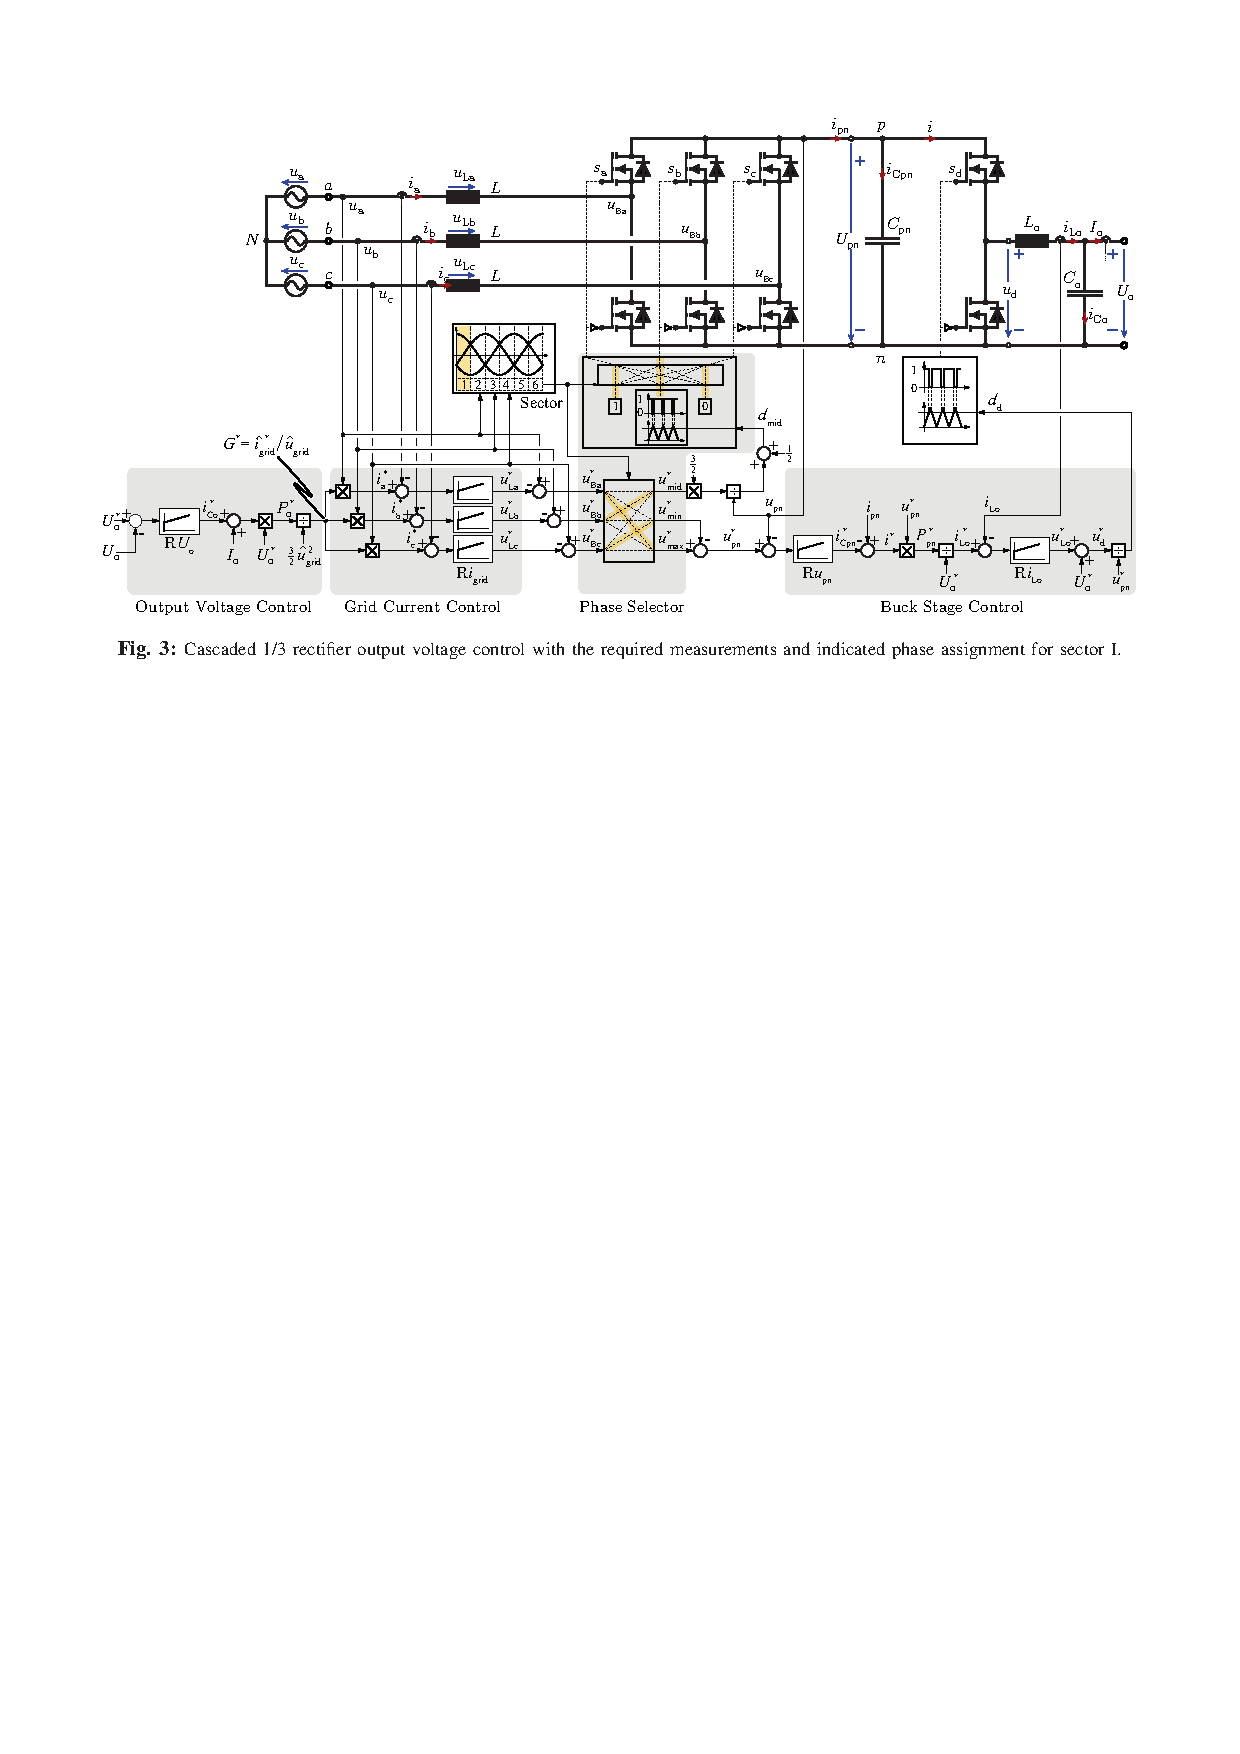
\includegraphics[width=0.65\linewidth]{content/Anhang/B6_Regelung}
	\caption{Regelungsstruktur des \gls{B6PFC} nach Menzi et Al. \cite{13PWMPFC}}
	\label{fig:b6regelung}
\end{figure}



\begin{table}
	\caption{Bewertungsmatrix der vier Simulierten Topologien}
\begin{tabular}{|c|c|c|c|c|c|}
	\hline
	Topologie & B6-1/3-PWM & Swiss & IAF & 6-Switch Buck & \% \\
	\hline
	L1 Netzinduktivität & 136 & 17,5 & 1 & 17,5 &\\
	\hline
	Gespeicherte Energie & 17,6 & 1,8 & 0,1 & 1,8 &\\
	\hline
	L2 DC Induktivität  & 136 & 136 & 136 & 136 &\\
	\hline
	Rippelstrom absolut & 88,5 & 88,5 & 88,5 & 88,5& \\
	\hline
	Gespeicherte Energie & 7,8 & 7,8 & 7,8 & 7,8 &\\
	\hline
	L3 IAF IVS Induktivität & - & - & 302,2 & - &\\
	\hline
	Gespeicherte Energie  & 0 & 0 & 8,82 & 0 &\\
	\hline
	Summe: & 225,52 & 9,6 & 16,8 & 9,6 &\\
	\hline
	\bfseries Induktivität normiert: & \bfseries 1 &\bfseries 0,38 &\bfseries 0,66 &\bfseries 0,38 & 50\\
	\hline
	C1 Netzkapazität & - & 50 & 50 & 50& \\
	\hline
	C2 am Elektrolyseur & 1 & 1 & 1 & 1 &\\
	\hline
	C3 DC Zwischenkreis & 25 & - & 50 & - &\\
	\hline
	\bfseries Kapazität normiert: &\bfseries 0,26 &\bfseries 0,5 &\bfseries 1 &\bfseries 0 &5\\
	\hline
	SiC 4mOhm & 0 & 0 & 2 & 0 &\\
	\hline
	SiC 2mOhm & 10 & 8 & 4 & 12 &\\
	\hline
	Vienna SiC 5mOhm & 0 & 6 & 6 & 0 &\\
	\hline
	\bfseries SiC normiert: &\bfseries 0,83 &\bfseries 0,87 &\bfseries 0,53 &\bfseries 1 &15\\
	\hline
	Vienna Diode & 0,0 & 6,0 & 6,0 & 0,0& \\
	\hline
	\bfseries Dioden normiert &\bfseries 0,0 & \bfseries1 &\bfseries 1 &\bfseries 0&5 \\
	\hline
	Treiberanzahl & 8 & 7 & 7 & 12 &\\
	\hline
	\bfseries Treiber normiert: &\bfseries 0,67 &\bfseries 0,58 &\bfseries 0,58 &\bfseries 1,00& 5\\
	\hline
	Schaltverluste 30 Grad & 567 & 215 & 503 & 303 &\\
	\hline
	Leitverluste 30 Grad & 254 & 1121 & 1311 & 543 &\\
	\hline
	Gewichtung 30 Grad & 75\% & 75\% & 75\% & 75\% &\\
	\hline
	Schaltverluste 0 Grad & 554 & 243 & 511 & 399& \\
	\hline
	Leitverluste 0 Grad & 326 & 781 & 748 & 722&\\
	\hline
	Gewichtung 0 Grad & 25\% & 25\% & 25\% & 25\%& \\
	\hline
	\bfseries Verluste normiert: &\bfseries 0,50 &\bfseries 0,75 &\bfseries 1,00 &\bfseries 0,55 &20\\
	\hline
	Gesamt &\bfseries 0,77 &\bfseries 0,57 &\bfseries 0,74 &\bfseries 0,52 & \\
	\hline
\end{tabular}
	\label{An:Entscheidungsmatrix}
\end{table}




		%Anhang hier einfügen
\end{document}